%%% Substrates

\def \CMPxcaa{(1-(benzyloxy)ethyl)benzene}		% methyl phenyl benzyl ether
\def \CMPxcab{($\pm$)-\textit{d}$_1$-(1-(benzyloxy)ethyl)benzene}		% methyl phenyl benzyl ether-d1
\def \CMPxcac{\textit{d}$_2$-(1-(benzyloxy)ethyl)benzene}		% methyl phenyl benzyl ether-d2

%%% Catalysts

\def \CMPxcad{imidazolium bromide salt}		% dicyclohexyl dibenzylated 
\def \CMPxcae{\textit{d}$_2$-imidazolium bromide salt}		% dicyclohexyl dibenzylated-d2
\def \CMPxcaf{imidazolium bromide salt}		% imes dibenzylated
\def \CMPxcag{imidazolium iodide salt}		% dicyclohexyl isopropyl iodide
\def \CMPxcah{imidazolium tetrafluoroborate salt}		% dicyclohexyl isopropyl bf4
\def \CMPxcai{imidazolium tetraphenylborate salt}		% dicyclohexyl isopropyl bph4
\def \CMPxcaj{imidazolium tetrakis[(3,5-trifluoromethyl)phenyl]\-borate salt}		% dicyclohexyl
% isopropyl barf
\def \CMPxcak{imidazolium chloride salt}		% dicyclohexyl-diOBn imidazolium chloride chiral
\def \CMPxcal{imidazolium ylide}		% dicyclohexyl dibenzylated ylide 
\def \CMPxcam{\textit{d}$_3$-imidazolium methoxide salt}		% dicyclohexyl dibenzylated methoxide salt
% d3
\def \CMPxcan{imidazolium bromide salt}		% dibenzyl 2-iPr
\def \CMPxcana{2,4,5-substituted imidazole}    % 2-iPr 4,5-dimethyl
\def \CMPxcanb{imidazolium chloride salt}    % dibenzyl 2-iPr 4,5-dimethyl


%%% Deuterated benzyl bromides

\def \CMPxcao{(\textit{R})-$\alpha$-deuterobenzyl bromide}		% d1 benzyl bromide
\def \CMPxcap{$\alpha$,$\alpha$-dideuterobenzyl bromide}		% d2 benzyl bromide
%\def \CMPxcaq{\textit{d}$_1$-benzyl alcohol}		% d1 benzyl alcohol
      % For compound systematic names

\subsection{General Information}

\subsubsection{General Procedures}
Unless stated otherwise, all reactions were carried out in flame-dried glassware under an atmosphere
of nitrogen passed through a tower of finely powdered Drierite\regtm\  in dry, degassed solvent with
standard Schlenk or vacuum-line techniques. Particularly air-sensitive manipulations were performed
in an MBraun Unilab nitrogen atmosphere glove box. Flash column chromatography was performed
according to the procedure of Still  \textit{et al.}\footnote{{\frenchspacing Still, W. C.; Kahn,
M.; Mitra, A. Rapid Chromatographic Technique for Preparative Separations with Moderate Resolution. \textit{J.
Org. Chem.} \textbf{1978}, \textit{43}, 2923-2925.}} with SiliCycle\regtm\
Silia\textit{Flash}\regtm\ P60 40-63 $\mu$m silica gel.
Analytical thin-layer chromatography (TLC) was performed using SiliCycle\regtm\  SiliaPlate 0.25 mm
silica gel 60 F254 plates. TLC plates were visualized by exposure to ultraviolet light and/or ceric ammonium
molybdate, \textit{p}-anisaldehyde, or potassium permanganate stains.

\subsubsection{Materials}
Toluene, tetrahydrofuran (THF), acetonitrile (\ce{CH3CN}),
dichloromethane (\ce{CH2Cl2}), and diethyl ether (\ce{Et2O}) were dispensed under nitrogen from a
Glass Contour solvent purification system custom manufactured by SG Waters, LLC (Nashua, NH). Deuterated chloroform
(\ce{CDCl3}), deuterated methanol (\ce{CD3OD}), and deuterated DMSO (DMSO-\textit{d}$_6$) were
purchased from Cambridge Isotope Labs and used as received. Deuterated benzene (\ce{C6D6}) and
deuterated toluene (toluene-\textit{d}$_8$) were purchased from Cambridge Isotope Labs and distilled
under nitrogen from \ce{CaCl2}. Molecular sieves (3\AA, 8-12
 mesh) were purchased from W.R.~Grace and activated by oven drying at 250
 \degc\ for at least 6 hours prior to use. Glyoxal (40\% in \ce{H2O}, w/w), 2-isopropylimidazole,
 paraformaldehyde, (1\textit{S},2\textit{S})-\textit{trans}-2-benzyloxycyclohexylamine,
 1,3-dicyclohexylimidazolium tetrafluoroborate, ammonium acetate (\ce{NH4OAc}), isobutyraldehyde,
 phosphorus tribromide (\ce{PBr3}), and \textit{N},\textit{N}-diisopropylethylamine (DIPEA) were
 purchased from Aldrich and used without further purification. Benzyl bromide and benzyl chloride
 were purchased from Aldrich, distilled from \ce{CaCl2} under reduced pressure, and stored under
 nitrogen in the dark at $-$20 \degc. Iodomethane was purchased from Aldrich, distilled under
 nitrogen, and stored over copper wire in the dark at $-$20 \degc. Sodium \textit{tert}-butoxide
 (NaOtBu) and potassium \textit{tert}-butoxide (KOtBu) were purchased from Aldrich and used as
 received inside a glove box.\footnote{Control reactions established there was no difference in
 reaction efficiency between sublimed material and unpurified commercial samples.} 2,3-Butanedione
 was purchased from Avocado Research Chemicals, fractionally distilled from \ce{MgSO4} under
 nitrogen, and stored in the dark at $-$20 \degc. 1-Phenylethanol was purchased from Aldrich,
 vacuum distilled from \ce{MgSO4}, and stored over 3\AA\ sieves (8-12 mesh). Potassium hydride (KH)
 was purchased from Strem Chemicals (20-25\% in oil) and was washed under nitrogen with excess
 pentane before storing in a glove box. Sodium tetrafluoroborate (Aldrich) and sodium
 tetraphenylborate (Lancaster) were vacuum dried (22 \degc, 18 h, approx.~1 mm Hg) over \ce{P2O5}
 before storing in a glove box. Sodium tetrakis[(3,5-trifluoromethyl)phenyl]borate
 (NaB(Ar$^\mathrm{F}$)$_4$) was prepared according to the literature procedure then vacuum dried (22 \degc, 18 h, approx.~1 mm Hg) over \ce{P2O5} before storing in a dry box.\footnote{{\frenchspacing Yakelis, N.
A.; Bergman, R.
G.
Safe Preparation and Purification of Sodium Tetrakis[(3,5-trifluoromethyl)phenyl]borate (NaBArF$_{24}$):
Reliable and Sensitive Analysis of Water in Solutions of Fluorinated Tetraarylborates. \textit{Organometallics} \textbf{2005}, \textit{24}, 3579-3581.}}
Ammonium chloride (\ce{NH4Cl}), concentrated hydrochloric acid (HCl), sodium carbonate
(\ce{Na2CO3}), potassium carbonate (\ce{K2CO3}), sodium sulfate (\ce{Na2SO4}), magnesium sulfate
(\ce{MgSO4}), ethyl acetate (EtOAc), glacial acetic acid (AcOH), ammonium hydroxide (\ce{NH4OH}),
and Celite\regtm\  545 were purchased from Fisher Scientific and used as received.

\subsubsection{Instrumentation}
Infrared spectra were recorded on a Bruker Alpha-p spectrometer. Bands are reported as strong (s),
medium (m), weak (w), broad strong (bs), broad medium (bm), and broad weak (bw). Optical rotation
data were recorded on a Rudolph research Autopol IV automatic polarimeter and has been reported as
the average of five readings. Melting points were recorded on a  Mel-Temp\regtm\  II manufactured by
Laboratory Devices, Inc.~and are uncorrected.
Sonication was performed with a Branson 1510 40 kHz bench-top sonicator. Microwave reactions were
performed in 10 mL sealed vessels with a CEM Discover\regtm\ 908005 system.  $^1$H NMR spectra were
recorded on a Varian VNMRS or Varian INOVA 500 MHz spectrometer.
Chemical shifts are reported in ppm from tetramethylsilane with the solvent resonance as the internal
standard (CHCl$_3$: $\delta$ 7.26, \ce{C6D6}: $\delta$ 7.16, \ce{CD3OD}: $\delta$ 3.31). Data are
reported as follows:
chemical shift, multiplicity (s = singlet, d = doublet, t = triplet, q = quartet, p = pentet, sept =
septet, dd = doublet of doublets, ddd = doublet of doublet of doublets, td = triplet of doublets,
qd = quartet of doublets, tt = triplet of triplets, m = multiplet), coupling constants (Hz), and
integration.
$^{13}$C NMR spectra were recorded on a Varian VNMRS 125 MHz spectrometer with complete proton
decoupling.
Chemical shifts are reported in ppm from tetramethylsilane with the solvent as the internal
reference (\ce{C6D6}: $\delta$ 128.06, CDCl$_3$: $\delta$ 77.16, \ce{CD3OD}: $\delta$ 49.00,
DMSO-\textit{d}$_6$:
$\delta$ 39.52). Gas chromatography (GC) analysis was performed on a Hewlett Packard HP 6890 system equipped with a flame ionization detector and HP-5
column (30 m x 0.320 mm x 0.25 $\mu$m) or Supelco\texttrademark~Beta DEX\texttrademark~120 column (30 m x 0.25 mm x 0.25 $\mu$m).
High-resolution mass spectra were obtained at the Boston College Mass Spectrometry Facility.


\pagebreak

%3.73 (dd, \textit{J} =  11.3, 4.1 Hz, 1H)
%\textit{J}$_{C\mbox{-}F}$
%%%%%%%%%%%%%%%%%%%%%%%%%%%%%%%%%%%%%%%%%%%%%%%%%%%%%%%%%%%%%%%%%%%%%%%%%%%%%%%%%%%%%%%%
% Begin experimental procedures for alkylation chapter.
%%%%%%%%%%%%%%%%%%%%%%%%%%%%%%%%%%%%%%%%%%%%%%%%%%%%%%%%%%%%%%%%%%%%%%%%%%%%%%%%%%%%%%%%
\subsection{Experimental Procedures and Characterization Data}
%% \noindent cannot be present directly under section headings
%***************[xcaa]%***************%
\begin{wrapfigure}{l}{1.05in}
  \vspace{-25pt}
  \begin{center}
    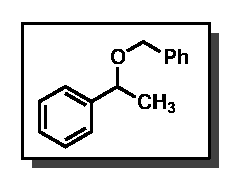
\includegraphics[scale=0.8]{chp_alkylation/images/xcaa}
  \end{center}
  \vspace{-30pt}
\end{wrapfigure}
\textit{Representative procedure for etherification of secondary alcohols
catalyzed by imidazolium salts:} \\ \textbf{\CMPxcaa}\ (\ref{cmp:xcaa}).
In a dry box, NaOtBu (21.1 mg, 0.220 mmol, 1.10 equiv) and imidazolium salt \ref{cmp:xcag} (8.0 mg,
0.020 mmol, 10 mol \%) were combined in a 1 dram (3.7 mL) vial. The mixture of solids was moved to
a nitrogen manifold and toluene (2 mL) was added, forming a white suspension. Benzyl bromide (36
$\mu$L, 0.30 mmol, 1.5 equiv) was added followed by 1-phenylethanol (24 $\mu$L, 0.20 mmol, 1.0
equiv). The reaction mixture was allowed to stir at room temperature for 2 hours and then quenched
by addition of \ce{Et2O} (1 mL) containing an accurately weighed quantity of
1,3,5-trimethoxybenzene.\footnote{A stock solution containing an accurately weighed quantity of
1,3,5-trimethoxybenzene in \ce{Et2O} was freshly prepared prior to workup. The stock solutions
typically contained 10.0-15.0 mg of 1,3,5-trimethoxybenzene per mL.} The reaction contents were
transferred to a 16 x 125 mm test tube containing saturated aqueous \ce{NH4Cl} (2 mL) and vigorously
stirred for 15 seconds. An aliquot of the upper organic layer was withdrawn and $^1$H NMR data were
obtained with a relaxation delay time of 10 seconds (d1 = 10). Integration of the internal standard
and product peaks indicated a yield of 0.16 mmol, 82\%. The highest yield obtained with imidazolium
salt \ref{cmp:xcag} was 0.18 mmol, 89\%. An analytically pure sample for comparison purposes was
obtained by purification on silica gel (5\% ethyl acetate in hexanes v/v) to afford a colorless oil.\\
R$_f$ = 0.64 (30\% ethyl acetate in hexanes); 
$^1$H NMR (CDCl$_3$, 500 MHz) $\delta$ 7.40-7.27 (m, 10H),  4.51 (q, \textit{J} = 6.6 Hz, 1H), 4.46
(d, \textit{J} = 11.7 Hz, 1H), 4.30 (d, \textit{J} = 12.0 Hz, 1H), 1.49 (d, \textit{J} = 6.6 Hz, 
3H); $^{13}$C NMR (CDCl$_3$, 125 MHz) $\delta$ 143.89, 138.81, 128.64, 128.49, 127.84, 127.64,
127.61, 126.49, 77.37, 70.45, 24.35; IR (neat) 3062 (bw), 3030 (bm), 2975 (bm), 2928 (bm), 2863
(bm), 1494 (m), 1452 (m), 1206 (m), 1095 (bm), 1053 (bm), 1028 (m), 912 (bw), 761 (m), 735 (m), 698
(s) cm$^{-1}$; HRMS (ESI+) Calcd.
for \ce{C15H20NO} [M+NH$_4$]$^+$:
230.1545; Found 230.1540.
% ***************[xcaa]%***************%

\vspace{10pt}
%***************[xcao]%***************%
\begin{wrapfigure}{l}{0.95in}
  \vspace{-25pt}
  \begin{center}
    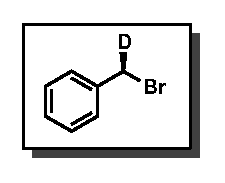
\includegraphics[scale=0.8]{chp_alkylation/images/xcao}
  \end{center}
  \vspace{-30pt}
\end{wrapfigure}
\noindent \textbf{\CMPxcao}\ (\ref{cmp:xcao}). A solution of (\textit{S})-$\alpha$-deuterobenzyl
alcohol\footnote{Prepared according to the procedure in reference \ref{ref:alknoyoritransfer}. The
material was obtained in 98:2 er as the \textit{S} enantiomer by Mosher's ester analysis. $\delta$ =
5.31 ppm (major), $\delta$ =
5.35 ppm (minor)} (750 mg, 6.87 mmol, 1.00 equiv) in 9.2 mL of \ce{CH2Cl2} was cooled to $-$78
\degc.
To the stirred solution, \ce{PBr3} (743 $\mu$L, 7.90 mmol, 1.15 equiv) was introduced dropwise \textit{via} syringe. The reaction mixture was stirred for 30 minutes at $-$78
\degc\ then poured into 25 mL of ice cold \ce{H2O}. The product was extracted with
\ce{CH2Cl2} (3 x 15 mL), dried over anhydrous \ce{Na2SO4} containing \ce{K2CO3}, filtered, and
concetrated to a colorless oil. The resulting oil was purified by K\"ugelrohr distillation under
reduced pressure to deliver \ref{cmp:xcao} as a colorless oil. The product was taken directly into
an inert atmosphere glove box and stored at $-$40 \degc\  in the dark.\\
\rotation = $+$0.160 (c 1.00,
\ce{CHCl3}); 
$^1$H NMR (CDCl$_3$, 500 MHz) $\delta$ 7.42-7.38 (m, 2H), 7.37-7.32 (m, 2H), 7.32-7.28 (m, 1H),
4.49 (t, \textit{J}$_{H\mbox{-}D}$ = 1.2 Hz, 1H); $^{13}$C NMR (CDCl$_3$, 125 MHz) $\delta$ 137.90,
129.18, 128.15, 128.57, 33.48 (t, \textit{J}$_{C\mbox{-}D}$ = 23.3 Hz); IR (neat)  3086
(bw), 3062 (bw), 3030 (bw), 1494 (m), 1452 (m), 1205 (m), 1163 (bm), 1074 (w), 882 (m),
742 (m), 691 (s) cm$^{-1}$.
% ***************[xcao]%***************%
\vspace{10pt}

%***************[xcab]%***************%
\begin{wrapfigure}{l}{1.05in}
  \vspace{-22pt}
  \begin{center}
    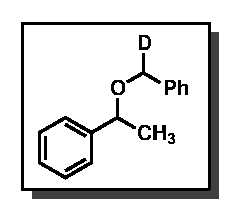
\includegraphics[scale=0.8]{chp_alkylation/images/xcab}
  \end{center}
  \vspace{-35pt}
\end{wrapfigure}
\noindent \textbf{\CMPxcab}\ (\ref{cmp:xcab}). In a glove box, KH (10.0 mg, 0.250 mmol, 1.00
equiv) was weighed into a 1 dram glass vial. The vial was removed from the glove box,
attached to a nitrogen manifold, and 1.5 mL of THF was added. To the stirred
suspension, 1-phenylethanol (30.5 mg, 0.250 mmol, 1.00 equiv) was added and the reaction mixture was
stirred for 10 minutes. After cooling to $-$78 \degc, ($\pm$)-\ref{cmp:xcao} (47.3 mg, 0.275 mmol, 1.10 equiv) dissolved in 1 mL of THF was
added in a single portion. The reaction mixture was allowed to warm slowly to room temperature
over 3 hours then poured into 15 mL of saturated aqueous \ce{NH4Cl}. The product was extracted with
\ce{Et2O} (3 x 15 mL), dried over anhydrous \ce{Na2SO4}, and concentrated to a colorless oil.
Purification by silica gel chromatography (5\% ethyl acetate in hexanes v/v) provided sufficient
material for comparison purposes as a colorless oil. Characterization data below were tabulated for the
1:1 mixture of diastereomers.
\\
R$_f$ = 0.64 (30\% ethyl acetate in hexanes); 
$^1$H NMR (CDCl$_3$, 500 MHz) $\delta$ 7.39-7.26 (m, 10H), 4.50 (q, \textit{J} = 6.4 Hz, 1H), 4.44
(t, \textit{J}$_{H\mbox{-}D}$ = 1.5 Hz, 0.5H), 4.28 (t, \textit{J}$_{H\mbox{-}D}$ = 1.5 Hz, 0.5H),
1.49 (d, \textit{J} = 6.4 Hz, 3H) ; $^{13}$C NMR (CDCl$_3$, 125 MHz) $\delta$ 143.90, 138.74,
128.64, 128.49, 127.86, 127.64, 127.62, 126.48, 77.32, 77.31, 70.11 (t, \textit{J}$_{C\mbox{-}D}$ = 21.9 Hz), 70.08 (t,
\textit{J}$_{C\mbox{-}D}$ = 21.4 Hz), 24.35; IR (neat) 3029 (bw), 2975 (bw), 2928 (bw),
2864 (bw), 1439 (w), 1450 (m), 1207 (w), 1096 (bs), 1057 (m), 1028 (m), 760 (m), 723 (m),
699 (s) cm$^{-1}$; HRMS (ESI+) Calcd.
for \ce{C15H19DNO} [M+NH$_4$]$^+$:
231.1608; Found 231.1616.
% ***************[xcab]%***************%


\vspace{10pt}
%***************[xcap]%***************%
\begin{wrapfigure}{l}{0.95in}
  \vspace{-25pt}
  \begin{center}
    
\includegraphics[scale=0.8]{chp_alkylation/images/xcap}
  \end{center}
  \vspace{-30pt}
\end{wrapfigure}
\noindent \textbf{\CMPxcap}\ (\ref{cmp:xcap}). Prepared in analogous fashion to \ref{cmp:xcao} with
$\alpha$,$\alpha$-dideuterobenzyl alcohol.
Characterization data were in agreement with the previously reported
values.\footnote{{\frenchspacing Miyashita, A.; Hotta, M.; Saida, Y. Selective sp$^3$ \ce{C-H} Bond Activation of Alkylaromatics
Promoted by Platinum Complexes. \textit{J. Organomet. Chem.} \textbf{1994}, \textit{473}, 353-358.}} \\
$^1$H NMR (CDCl$_3$, 500 MHz) $\delta$ 7.42-7.38 (m, 2H), 7.37-7.33 (m, 2H), 7.32-7.28 (m, 1H); 
$^{13}$C NMR (CDCl$_3$, 125 MHz) $\delta$ 137.80, 129.13, 128.91, 128.54, 33.24 (p,
\textit{J}$_{C\mbox{-}D}$ = 23.3 Hz).
% ***************[xcap]%***************%

\vspace{10pt}
%***************[xcac]%***************%
\begin{wrapfigure}{l}{1.1in}
  \vspace{-22pt}
  \begin{center}
    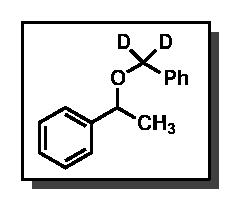
\includegraphics[scale=0.8]{chp_alkylation/images/xcac}
  \end{center}
  \vspace{-30pt}
\end{wrapfigure}
\noindent \textbf{\CMPxcac}\ (\ref{cmp:xcac}). Prepared according to the procedure for
\ref{cmp:xcab} with \CMPxcap~(\ref{cmp:xcap}) to afford a colorless oil.\\
R$_f$ = 0.64 (30\% ethyl acetate in hexanes); 
$^1$H NMR (CDCl$_3$, 500 MHz) $\delta$ 7.41-7.28 (m, 10H), 4.52 (q, \textit{J} = 6.6 Hz, 1H), 1.51
(d, \textit{J} = 6.4 Hz, 3H); $^{13}$C NMR (CDCl$_3$, 125 MHz) $\delta$ 143.90, 138.68, 128.63,
128.49, 127.88, 127.63, 126.48, 77.25, 24.34; IR (neat) 3028 (bw), 2975 (bw), 2928 (bw), 2862 (bw), 1493 (m), 1448 (m), 1370 (w),
1207 (w), 1096 (bs), 1025 (bm), 759 (m), 697 (s) cm$^{-1}$; HRMS (ESI+) Calcd. for \ce{C15H18D2NO}
[M+NH$_4$]$^+$:
232.1670; Found 232.1664.
% ***************[xcac]%***************%

\pagebreak
%***************[xcad]%***************%
\begin{wrapfigure}{l}{1.40in}
  \vspace{-12pt}
  \begin{center}
    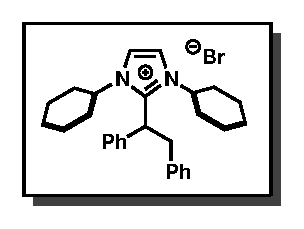
\includegraphics[scale=0.8]{chp_alkylation/images/xcad}
  \end{center}
  \vspace{-25pt}
\end{wrapfigure}
\noindent \textbf{\CMPxcad}\ (\ref{cmp:xcad}). In a glove box 1,3-dicyclohexylimidazolium
tetrafluoroborate (320 mg, 1.00 mmol, 1.00 equiv) was combined with KOtBu (241 mg, 2.15 mmol, 2.15
equiv). The mixture of solids was moved to a nitrogen manifold, suspended in THF (20 mL) and placed
in a sonication bath for 1 minute to form a clear homogenous solution.
Benzyl bromide (250 $\mu$L, 2.05 mmol, 2.05 equiv) was introduced dropwise causing the immediate
formation of a white precipitate. The yellow reaction mixture was sonicated at 45 \degc\ for 24
hours then cooled to room temperature and filtered through
Celite$\textsuperscript{\textregistered}$ 545, rinsing with excess \ce{CH2Cl2}. Concentration
afforded a pale yellow solid that was recrystallized by slow vapor diffusion of \ce{Et2O} into a
\ce{CH2Cl2} solution to provide \ref{cmp:xcad} as a white solid (487 mg, 98.7\%), mp 166-168 \degc.
\\
$^1$H NMR (\ce{CD3OD}, 500 MHz) $\delta$ 7.73 (s, 2H), 7.54-7.48 (m, 2H), 7.44-7.39 (m, 3H),
7.35-7.30 (m, 2H), 7.30-7.25 (m, 1H), 7.18-7.14 (m, 2H), 5.52 (dd, \textit{J} = 12.7, 4.2 Hz, 1H),
4.15-4.02 (m, 2H), 3.39 (dd, \textit{J} = 13.2, 4.4 Hz, 1H), 3.45 (t, \textit{J} = 13.0 Hz,
1H), 2.18-2.10 (m, 2H), 1.96-1.89 (m, 2H), 1.88-1.76 (m, 2H), 1.68-1.60 (m, 2H), 1.59-1.46 (m, 4H),
1.40-1.29 (qd, \textit{J} = 12.5, 3.7 Hz, 2H), 1.27-1.15 (m, 2H), 1.02-0.84 (m,
2H), 0.52-0.35 (m, 2H); $^{13}$C NMR (CD$_3$OD, 125 MHz) $\delta$ 146.24, 138.71, 138.52, 130.58, 130.32, 130.22, 129.38, 128.64, 128.58, 120.99, 59.50, 43.16, 37.98, 34.60, 33.18, 26.32, 26.26, 25.55; IR (neat) 3027 (bw), 2929 (bm), 2855 (bw), 1573 (bw), 1495 (m), 1450 (m), 1196 (bw), 1030 (bw), 896 (m), 744 (m), 722 (m), 698 (s) cm$^{-1}$; HRMS (ESI+) Calcd.
for \ce{C29H37N2} [M]$^+$:
413.2957; Found 413.2960.
% ***************[xcad]%***************%

\vspace{10pt}
%***************[xcae]%***************%
\begin{wrapfigure}{l}{1.35in}
  \vspace{-25pt}
  \begin{center}
    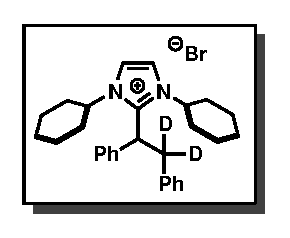
\includegraphics[scale=0.8]{chp_alkylation/images/xcae}
  \end{center}
  \vspace{-30pt}
\end{wrapfigure}
\noindent \textbf{\CMPxcae}\ (\ref{cmp:xcae}). An authentic sample for comparison purposes was
prepared according the procedure for imidazolium salt \ref{cmp:xcad} with
$\alpha$,$\alpha$-dideuterobenzyl bromide.
The material recovered contained approximately 60\% proton incorporation at the benzylic methine
position by $^1$H NMR spectroscopy. There also appeared to be some deuterium incorporation on the
backbone. The $^{13}$C NMR data were difficult to deconvolute and have been tabulated below for the
mixture of compounds.
\\
$^1$H NMR (CD$_3$OD, 500 MHz) $\delta$ 7.72 (s, 2H), 7.53-7.48 (m, 2H), 7.44-7.39 (m, 3H),
7.35-7.25 (m, 3H), 7.17-7.13 (m, 2H), 5.50 (s, 1H), 4.14-4.03 (m, 2H), 2.20-2.11 (m, 2H), 1.97-1.88
(m, 2H), 1.88-1.74 (m, 2H), 1.68-1.60 (m, 2H), 1.60-1.46 (m, 4H), 1.33 (qd, \textit{J} = 12.5, 3.7 Hz, 2H), 1.26-1.15 (m, 2H), 1.00-0.84 (m, 2H), 0.53-0.34 (m, 2H); $^{13}$C NMR
(CD$_3$OD, 125 MHz) $\delta$ 146.20, 146.16, 138.62, 138.51, 138.44, 130.56, 130.29, 130.20,
129.35, 129.34, 128.60, 128.58, 121.01, 120.89, 59.46, 43.00, 34.56, 33.17, 26.30, 26.26, 25.54;
HRMS (ESI+) Calcd.
for \ce{C29H35D2N2} [M]$^+$:
415.3077; Found 415.3072.
% ***************[xcae]%***************%

\vspace{10pt}
%***************[xcaf]%***************%
\begin{wrapfigure}{l}{1.6in}
  \vspace{-25pt}
  \begin{center}
    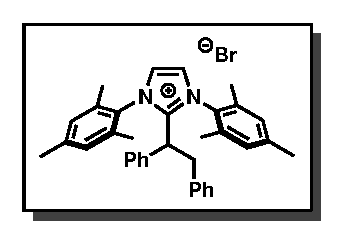
\includegraphics[scale=0.8]{chp_alkylation/images/xcaf}
  \end{center}
  \vspace{-30pt}
\end{wrapfigure}
\noindent \textbf{\CMPxcaf}\ (\ref{cmp:xcaf}). Prepared according to the procedure for imidazolium
bromide \ref{cmp:xcad} on 0.300 mmol scale. The product was recrystallized by slow vapor diffusion
of hexanes into a saturated \ce{CHCl3} solution at $-$20 \degc\  to afford \ref{cmp:xcaf} as a white
solid (151 mg, 89.1\%), mp 219-223 \degc.
\\
$^1$H NMR (CDCl$_3$, 500 MHz) $\delta$ 8.29 (s, 2H), 7.20-7.13 (m, 3H), 7.06-6.99 (m, 7H),
6.62-6.58 (m, 2H), 6.47-6.43 (m, 2H), 4.28 (dd, \textit{J} = 12.5, 3.4 Hz, 1H), 3.26-3.14 (m, 2H),
2.45 (s, 6H), 2.19 (s, 6H), 1.79 (s, 6H); $^{13}$C NMR (CDCl$_3$, 125 MHz) $\delta$ 146.46, 142.19, 135.65, 135.18, 134.51,
131.05, 130.33, 130.21, 130.15, 129.18, 128.91, 128.57, 128.53, 128.26, 127.10, 126.53, 44.19, 35.95, 21.22, 18.08, 17.41; IR (neat) 3056 (bw), 3022 (bw), 2992 (bw), 2919 (bw), 1605 (w), 1559 (w), 1494 (s),
1453 (m), 1382 (w), 1239 (m), 1034 (bw), 859 (m), 792 (m), 752 (m), 696 (s) cm$^{-1}$; HRMS (ESI+)
Calcd.
for \ce{C35H37N2} [M]$^+$:
485.2957; Found 485.2976.
% ***************[xcaf]%***************%

\vspace{10pt}
%***************[xcag]%***************%
\begin{wrapfigure}{l}{1.35in}
  \vspace{-25pt}
  \begin{center}
    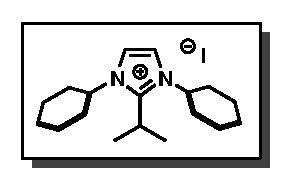
\includegraphics[scale=0.8]{chp_alkylation/images/xcag}
  \end{center}
  \vspace{-30pt}
\end{wrapfigure}
\noindent \textbf{\CMPxcag}\ (\ref{cmp:xcag}). In a glove box 1,3-dicyclohexylimidazolium
tetrafluoroborate (1.60 g, 5.00 mmol, 1.00 equiv) was combined with KOtBu (2.24 g, 20.0 mmol, 4.00
equiv). The mixture of solids was moved to a nitrogen manifold, suspended in THF (50 mL), and placed
in a sonication bath for 1 minute to form a clear homogenous solution.
Iodomethane (1.56 mL, 25.0 mmol, 5.00 equiv) was introduced dropwise causing the immediate
formation of a white precipitate. The reaction mixture was sonicated at 45 \degc\ for 3 days  then
cooled to room temperature and filtered through Celite$\textsuperscript{\textregistered}$ 545, rinsing with excess \ce{CH2Cl2}. Concentration
afforded a pale yellow solid that was recrystallized by slow vapor diffusion of \ce{Et2O} into a
\ce{CHCl3} solution to provide \ref{cmp:xcag} as a faint yellow solid (1.80 g, 89.5\%), mp $>$250
\degc~(decomp).\\
$^1$H NMR (\ce{CD3OD}, 500 MHz) $\delta$ 7.75 (s, 2H), 4.47 (tt, \textit{J} = 12.0, 3.8 Hz, 2H),
3.89 (sept, \textit{J} = 7.4 Hz, 1H), 2.07-2.00 (m, 4H), 1.97-1.91 (m, 4H), 1.84 (qd, \textit{J}
= 12.4, 3.6 Hz, 4H), 1.80-1.74 (m, 2H), 1.65-1.54 (m, 4H), 1.51 (d, \textit{J} = 7.2 Hz,
6H), 1.42-1.31 (m, 2H); $^{13}$C NMR (CD$_3$OD, 125 MHz) $\delta$ 149.60, 120.57, 59.37, 34.39, 26.24, 25.79, 25.73, 19.99; IR (neat)  3085 (bw), 3053 (bw), 2925 (bs), 2859 (m), 1573 (w), 1501 (m), 1449 (m), 3838 (w), 1252 (m), 1201 (s), 1145 (w), 1100 (m), 1002 (w), 985 (w), 896 (m), 785 (m), 752 (m),
738 (m) cm$^{-1}$; HRMS (ESI+) Calcd.
for \ce{C18H31N2} [M]$^+$:
275.2487; Found 275.2501.
% ***************[xcag]%***************%

\vspace{10pt}
%***************[xcah]%***************%
\begin{wrapfigure}{l}{1.35in}
  \vspace{-25pt}
  \begin{center}
    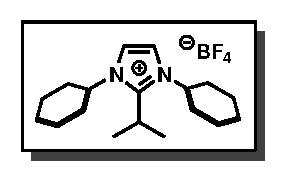
\includegraphics[scale=0.8]{chp_alkylation/images/xcah}
  \end{center}
  \vspace{-30pt}
\end{wrapfigure}
\noindent \textbf{\CMPxcah}\ (\ref{cmp:xcah}). In a glove box, imidazolium iodide \ref{cmp:xcag}
(101 mg, 0.250 mmol, 1.00 equiv) was dissolved in 2.5 mL of \ce{CH2Cl2}. To the stirred solution,
\ce{NaBF4} (27.4 mg, 0.250 mmol, 1.00 equiv) was added as a solid in a single portion. The
suspension was stirred for 2 days then filtered through glass wool and concentrated \textit{in
vacuo}.
The resulting white solid was suspended in 2 mL of hexanes and concentrated again to afford \ref{cmp:xcah} as a
white powder (81.0 mg, 89.4\%), mp 246-250 \degc~(decomp). 
\\
$^1$H NMR (CD$_3$OD, 500 MHz) $\delta$ 7.74 (s, 2H), 4.45 (tt, \textit{J} = 12.0, 3.9 Hz, 2H), 3.87
(sept, \textit{J} = 6.9 Hz, 1H), 2.06-2.00 (m, 4H), 1.98-1.90 (m, 4H), 1.89-1.74 (m, 6H),
1.64-1.53 (m, 4H), 1.51 (d, \textit{J} = 7.3 Hz, 6H), 1.41-1.31 (m, 2H); $^{13}$C NMR (CD$_3$OD, 125
MHz) $\delta$ 149.60, 120.52, 59.38, 34.37, 26.24, 25.78, 25.73, 19.90; IR (neat)  3084 (bw), 3051 (bw), 2926 (bm), 2860 (bm), 1574 (w), 1500 (m), 1450 (m), 1253 (w), 1201 (m), 1144 (bw), 1098 (bm), 1056 (bs), 897 (m), 784 (m), 753 (m), 737 (m) cm$^{-1}$; HRMS
(ESI+) Calcd.
for \ce{C18H31N2} [M]$^+$:
275.2487; Found 275.2489.
% ***************[xcah]%***************%

\vspace{10pt}
%***************[xcai]%***************%
\begin{wrapfigure}{l}{1.35in}
  \vspace{-25pt}
  \begin{center}
    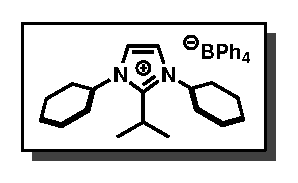
\includegraphics[scale=0.8]{chp_alkylation/images/xcai}
  \end{center}
  \vspace{-30pt}
\end{wrapfigure}
\noindent \textbf{\CMPxcai}\ (\ref{cmp:xcai}). Prepared according to the procedure for
\ref{cmp:xcah} on 0.250 mmol scale with \ce{NaBPh4} (85.6 mg, 0.250 mmol, 1.00 equiv) to afford
\ref{cmp:xcai} as a white solid (136 mg, 91.3\%), mp 179-182 \degc.\\
$^1$H NMR (CDCl$_3$, 500 MHz) $\delta$ 7.46-7.40 (m, 8H), 7.04 (t, \textit{J} = 7.3 Hz, 8H), 6.90
(t, \textit{J} = 7.1 Hz, 4H), 6.08 (s, 2H), 3.91 (tt, \textit{J} = 12.2, 3.4 Hz, 2H), 3.33 (sept,
\textit{J} = 7.1 Hz, 1H), 1.99-1.91 (m, 4H), 1.79-1.69 (m, 6H), 1.51-1.41 (m, 4H), 1.37 (d,
\textit{J} = 7.3 Hz, 6H), 1.36-1.24 (m, 6H); $^{13}$C NMR (DMSO-\textit{d}$_6$, 125 MHz) $\delta$
163.35 (q, \textit{J}$_{C\mbox{-}B}$ = 49.4 Hz), 147.65, 135.52, 135.51, 125.22 (q, \textit{J}$_{C\mbox{-}B}$ = 2.4 Hz), 121.45, 119.44, 56.94, 32.54, 24.57, 24.24, 23.55, 19.11; IR (neat) 3054 (bw), 2982 (bw), 2928 (bw), 2857 (bw), 1578 (w), 1495 (w), 1477 (bw), 1449 (w), 1223 (w), 1267 (bw), 1189 (w), 1131 (bw), 1096
(bw), 894 (w), 843 (w), 734 (m), 701 (s), 611 (m) cm$^{-1}$; HRMS (ESI+) Calcd.
for \ce{C18H31N2} [M]$^+$:
275.2487; Found 275.2492.
% ***************[xcai]%***************%

\vspace{10pt}
%***************[xcaj]%***************%
\begin{wrapfigure}{l}{2.0in}
  \vspace{-20pt}
  \begin{center}
    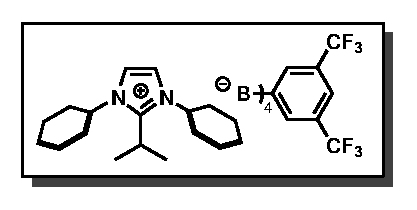
\includegraphics[scale=0.8]{chp_alkylation/images/xcaj}
  \end{center}
  \vspace{-30pt}
\end{wrapfigure}
\noindent \textbf{\CMPxcaj}\ (\ref{cmp:xcaj}). Prepared according to the procedure for
\ref{cmp:xcah} on 0.250 mmol scale with NaB(Ar$^\mathrm{F}$)$_4$ (222 mg, 0.250 mmol, 1.00 equiv) to
afford \ref{cmp:xcaj} as a white solid (218 mg, 76.6\%), mp 152-155 \degc.\\
$^1$H NMR (CD$_3$OD, 500 MHz) $\delta$ 7.69 (s, 2H), 7.63-7.58 (m, 12H), 4.38 (tt, \textit{J} =
12.0, 3.7 Hz, 2H), 3.77 (sept, \textit{J} = 7.3 Hz, 1H), 2.02-1.95 (m, 4H), 1.94-1.87 (m, 4H),
1.83-1.70 (m, 6H), 1.57-1.46 (m, 4H), 1.46 (d, \textit{J} = 7.3 Hz, 6H), 1.36-1.23 (m, 2H); $^{13}$C
NMR (CD$_3$OD, 125 MHz) $\delta$ 162.90 (q, \textit{J}$_{C\mbox{-}B}$ = 49.8 Hz), 149.56, 135.84,
130.47 (qq, \textit{J}$_{C\mbox{-}F\mbox{-}B}$ = 31.4, 3.3 Hz), 125.79 (q, \textit{J}$_{C\mbox{-}F}$
= 271.7 Hz), 120.44, 118.50 (broad), 59.47, 34.36, 26.21, 25.79, 25.69, 19.70; IR (neat) 2947 (bw),
2870 (bw), 1610 (bw), 1495 (bw), 1454 (bw), 1353 (m), 1273 (s), 1159 (bm), 1114 (bs), 887 (m), 838 (m), 715 (m), 682 (m), 668 (m) cm$^{-1}$; HRMS (ESI+) Calcd. for \ce{C18H31N2} [M]$^+$:
275.2487; Found 275.2491.
% ***************[xcaj]%***************%

\vspace{10pt}
%***************[xcak]%***************%
\begin{wrapfigure}{l}{1.45in}
  \vspace{-18pt}
  \begin{center}
    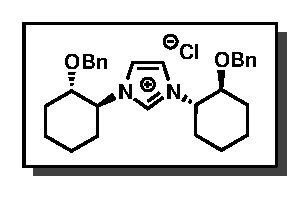
\includegraphics[scale=0.8]{chp_alkylation/images/xcak}
  \end{center}
  \vspace{-30pt}
\end{wrapfigure}
\noindent \textbf{\CMPxcak}\ (\ref{cmp:xcak}). A solution of (1\textit{S},2\textit{S})-\textit{trans}-2-benzyloxycyclohexylamine (205 mg, 1.00 mmol, 2.00 equiv) in toluene (4 mL) was cooled to 0 \degc. Paraformaldehyde (15.0 mg, 0.500 mmol, 1.00 equiv) was added as a
solid in a single portion and the reaction mixture was stirred for 20 minutes. Concentrated HCl
(41.8 $\mu$L, 0.500 mmol, 1.00 equiv, 12 N) and glyoxal (57.1 $\mu$L, 0.500 mmol, 1.00 equiv, 40.0\%
 w/w in water) were added at 0 \degc\  then the mixture was warmed to reflux and heated for 46
 hours.
 After cooling to room temperature, 30 mL of saturated aqueous \ce{Na2CO3} was added. The
aqueous layer was washed with EtOAc (3 x 20 mL) and the organic washes were discarded. The
product was extracted with \ce{CH2Cl2} (6 x 30 mL) and the combined organics were dried over
\ce{MgSO4}, filtered, and concentrated to afford \ref{cmp:xcak} as a white solid (205 mg,
85.3\%), mp 134-137 \degc.\\
\rotation = $+$110.0 (c 0.94, \ce{CHCl3});
$^1$H NMR (CD$_3$OD, 500 MHz) $\delta$ 9.03 (t, \textit{J} = 1.7 Hz, 1H), 7.63 (d, \textit{J} =
1.7 Hz, 2H), 7.26-7.21 (m, 6H), 7.04-7.00 (m, 4H), 4.51 (d, \textit{J} = 12.0 Hz, 2H), 4.19 (ddd,
\textit{J} = 12.2, 10.0, 4.4 Hz, 2H), 4.14 (d, \textit{J} = 11.7 Hz, 2H), 3.53 (td, \textit{J} =
10.5, 4.6 Hz, 2H), 2.43-2.36 (m, 2H), 2.11-2.04 (m, 2H), 1.97-1.85 (m, 6H), 1.54-1.27 (m, 6H); $^{13}$C NMR (CD$_3$OD, 125 MHz) $\delta$ 139.32, 136.90, 129.40, 128.75, 128.70, 121.76, 121.72, 80.32, 71.44, 65.52, 65.50, 32.26, 32.25, 31.66, 25.60, 24.62; IR (neat)  3033 (bw), 2933 (bm), 2859 (bm), 1554 (bw), 1451 (m), 1361 (bw), 1169 (m), 1095 (bs), 1028 (m), 941 (m), 870 (m), 800 (w), 734 (s), 696 (s), 658 (m) cm$^{-1}$; HRMS (ESI+) Calcd.
for \ce{C29H37N2O2} [M]$^+$:
445.2855; Found 445.2837.
% ***************[xcak]%***************%

\vspace{10pt}
%***************[xcal]%***************%
\begin{wrapfigure}{l}{1.35in}
  \vspace{-33pt}
  \begin{center}
    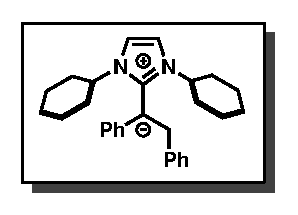
\includegraphics[scale=0.8]{chp_alkylation/images/xcal}
  \end{center}
  \vspace{-30pt}
\end{wrapfigure}
\noindent \textbf{\CMPxcal}\ (\ref{cmp:xcal}). In a glove box, imidazolium salt \ref{cmp:xcad}
(150 mg, 0.300 mmol, 1.00 equiv) was suspended in 5 mL of toluene. To the stirred suspension, NaOtBu
(27.5 mg, 0.286 mmol, 0.95 equiv) was added as a solid in a single portion, causing an immediate
yellow coloration.
The reaction mixture was stirred for 24 hours then filtered through Celite\regtm\  545 and concentrated under high vacuum
to afford \ref{cmp:xcal} as a sensitive dark green solid (83.2 mg, 70.5\%).
\\
$^1$H NMR (C$_6$D$_6$, 500 MHz) $\delta$ 7.46 (d, \textit{J} = 7.3 Hz, 2H), 7.27 (dd, \textit{J} =
8.6, 1.0 Hz, 2H), 7.20-7.16 (m, 2H), 7.12 (dd, \textit{J} = 7.6, 7.6 Hz, 2H), 7.03-6.99 (m, 1H),
6.77 (tt, \textit{J} = 7.1, 1.2 Hz, 1H), 6.02 (s, 2H), 4.14 (s, 2H), 3.79 (tt, \textit{J} = 11.7,
3.4 Hz, 2H), 1.89-1.82 (m, 4H), 1.49-1.42 (m, 4H), 1.30-1.24 (m, 2H), 1.14-1.03 (m, 4H), 0.88-0.76
(m, 6H); $^{13}$C NMR (C$_6$D$_6$, 125 MHz) $\delta$ 152.42, 145.90, 144.31, 128.79, 128.66, 128.37,
128.25, 127.97, 127.87, 125.57, 122.70, 118.33, 113.94, 69.00, 57.15, 38.85, 32.61, 25.87, 25.76; IR
(neat)  3132 (bw), 3054 (bw), 3017 (bw), 2926 (bs), 2852 (m), 1671 (bw), 1521 (s), 1485
(s), 1446 (m), 1379 (m), 1269 (s), 1177 (s), 964 (m), 892 (m), 758 (m), 729 (m), 694 (s),
631 (m), 602 (m) cm$^{-1}$.
% ***************[xcal]%***************%

\vspace{10pt}
%***************[xcam]%***************%
\begin{wrapfigure}{l}{1.55in}
  \vspace{-25pt}
  \begin{center}
    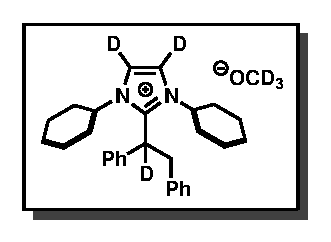
\includegraphics[scale=0.8]{chp_alkylation/images/xcam}
  \end{center}
  \vspace{-30pt}
\end{wrapfigure}
\noindent \textbf{\CMPxcam}\ (\ref{cmp:xcam}). A sample of imidazolium ylide \ref{cmp:xcal}
(approx.~25 mg) was dissolved in 1 mL of \ce{CD3OD} to give a clear colorless solution. The solution was concentrated
under high vacuum and the resulting colorless oil was re-dissolved in 0.7 mL of \ce{CD3OD} for
spectral analysis.
\\ 
$^1$H NMR (CD$_3$OD, 500 MHz) $\delta$ 7.53-7.49 (m, 2H), 7.45-7.38 (m, 3H), 7.35-7.26 (m, 3H),
7.16-7.13 (m, 2H), 4.13-4.02 (m, 2H), 3.92 (d, \textit{J} = 13.2 Hz, 1H), 3.44 (d, \textit{J} =
13.2 Hz, 1H), 2.18-2.11 (m, 2H), 1.96-1.89 (m, 2H), 1.86-1.73 (m, 2H), 1.68-1.61 (m, 2H), 1.59-1.44
(m, 4H), 1.32 (qd, \textit{J} = 12.5, 3.9 Hz, 2H), 1.25-1.14 (m, 2H), 1.00-0.83 (m,
2H), 0.49-0.35 (m, 2H); $^{13}$C NMR (CD$_3$OD, 125 MHz) $\delta$ 146.22, 138.71, 138.47, 130.62,
130.35, 130.19, 129.46, 128.69, 128.57, 120.62 (t, \textit{J}$_{C\mbox{-}D}$ = 22.9 Hz), 59.51,
42.86 (t, \textit{J}$_{C\mbox{-}D}$ = 20.1 Hz), 37.89, 34.60 (broad), 33.20, 26.34, 26.27, 25.58;
HRMS (ESI+) Calcd.
for \ce{C29H34D3N2} [M]$^+$:
416.3140;  Found 416.3155.
% ***************[xcam]%***************%

\vspace{10pt}
%***************[xcan]%***************%
\begin{wrapfigure}{l}{1.65in}
  \vspace{-30pt}
  \begin{center}
    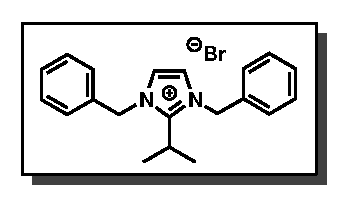
\includegraphics[scale=0.8]{chp_alkylation/images/xcan}
  \end{center}
  \vspace{-35pt}
\end{wrapfigure}
\noindent \textbf{\CMPxcan}\ (\ref{cmp:xcan}). To a suspension of 2-isopropylimidazole (220 mg,
2.00 mmol, 1.00 equiv) and \ce{K2CO3} (1.10 g, 8.00 mmol, 4.00 equiv) in THF (10 mL), benzyl
bromide (977 $\mu$L, 8.00 mmol, 4.00 equiv) was added in a single portion. The reaction mixture
was refluxed for 20 hours then cooled to room temperature and diluted with 10 mL of 1:1 \ce{CH2Cl2}:
 \ce{CH3OH} (v/v). The suspension was filtered through Celite\regtm~545, concentrated, and
recrystallized from minimal \ce{CH3CN} and EtOAc (approx.~5:1 v/v) to afford \ref{cmp:xcan} as a
white solid (500 mg, 67.4\%), mp 158-160 \degc.\\
$^1$H NMR (CD$_3$OD, 500 MHz) $\delta$ 7.58 (s, 2H), 7.47-7.38 (m, 6H), 7.33-7.29 (m, 4H), 5.58 (s,
4H), 3.77 (sept, \textit{J} = 7.3 Hz, 1H), 1.29 (d, \textit{J} = 7.3 Hz, 6H); $^{13}$C NMR
(CD$_3$OD, 125 MHz) $\delta$ 151.79, 135.57, 130.41, 129.98, 128.56, 124.05, 53.33, 26.70, 19.15; IR (neat)  3062 (bw), 2972 (bw), 2876 (bw), 1579 (w), 1513 (w), 1371 (bw), 1260 (w),
1174 (w), 789 (bw), 728 (s), 697 (bm) cm$^{-1}$; HRMS (ESI+) Calcd. for \ce{C20H23N2} [M]$^+$: 291.1861;
Found 291.1874.
% ***************[xcan]%***************%

\vspace{10pt}
%***************[xcana]%***************%
\begin{wrapfigure}{l}{0.95in}
  \vspace{-25pt}
  \begin{center}
    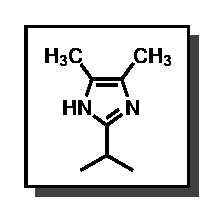
\includegraphics[scale=0.8]{chp_alkylation/images/xcana}
     \begin{textblock}{1}(0.2,-1.15) \cmp{xcana} \end{textblock}
  \end{center}
  \vspace{-30pt}
\end{wrapfigure}
\noindent \textbf{\CMPxcana}\ (\ref{cmp:xcana}). In a microwave vessel, 2,3-butanedione (104 $\mu$L, 1.20 mmol, 1.00 equiv), isobutyraldehyde (110
$\mu$L, 1.20 mmol, 1.00 equiv), and \ce{NH4OAc} (925 mg, 12.0
mmol, 10.0 equiv) were suspended in glacial AcOH (2.5 mL). The reaction
mixture was microwaved at 180 \degc\ for 5 minutes then rapidly cooled to room temperature. The
reaction contents were transferred carefully to a solution of saturated aqueous \ce{NH4OH} (15 mL)
that was chilled to 0 \degc. The product was extracted with \ce{CH2Cl2} (3 x 25 mL), dried over
\ce{MgSO4}, filtered, and concentrated to a pale yellow solid. The solid was dissolved in minimal
warm 1:1 \ce{Et2O}: hexanes (v/v), cooled to $-$20 \degc, filtered, and washed with hexanes to
afford \ref{cmp:xcana} as a faint yellow solid (81.0 mg, 48.8\%), mp 194-196 \degc.
\\
$^1$H NMR (CDCl$_3$, 500 MHz) $\delta$ 8.33 (broad s, 1H), 2.97 (sept, \textit{J} = 7.1 Hz, 1H),
2.13 (s, 6H), 1.3 (d, \textit{J} = 7.1 Hz, 6H); $^{13}$C NMR (CDCl$_3$, 125 MHz) $\delta$ 151.15,
125.56 (broad), 28.35, 21.98, 10.76; IR (neat) 3157 (bw), 2964 (m), 2916 (bm), 2872 (bm), 1620 (m),
1438 (bs), 1390 (m), 1287 (bm), 1096 (m), 1019 (m), 884 (bw), 735 (w) cm$^{-1}$; HRMS (ESI+) Calcd.
for \ce{C8H15N2} [M+H]$^+$:
139.1235; Found 139.1230.
% ***************[xcana]%***************%

\pagebreak
%***************[xcanb]%***************%
\begin{wrapfigure}{l}{1.6in}
  \vspace{-15pt}
  \begin{center}
    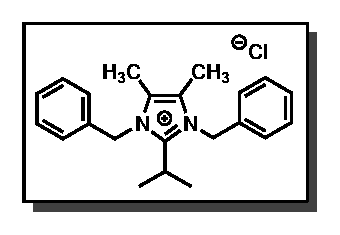
\includegraphics[scale=0.8]{chp_alkylation/images/xcanb}
  \end{center}
  \vspace{-30pt}
\end{wrapfigure}
\noindent \textbf{\CMPxcanb}\ (\ref{cmp:xcanb}). In a microwave vessel, imidazole \ref{cmp:xcana}
(41.5 mg, 0.300 mmol, 1.00 equiv), DIPEA (78.4 $\mu$L, 0.450 mmol, 1.50 equiv), and benzyl chloride (173
$\mu$L, 1.50 mmol, 5.00 equiv) were dissolved in \ce{CH3CN} (1.5 mL). The reaction
mixture was microwaved at 180 \degc\ for 5 minutes then rapidly cooled to room temperature. The
solvent was removed \textit{in vacuo} and resulting dark brown oil was dissolved in 50 mL of
saturated aqueous \ce{K2CO3}. The aqueous solution was washed with \ce{Et2O} (2 x 25 mL),
discarding the organic washes. The product was extracted with \ce{CH2Cl2} (3 x 75 mL), dried over
\ce{MgSO4}, filtered, and concentrated to afford \ref{cmp:xcanb} as a white solid (36.2 mg,
34.0\%), mp 138-140 \degc.\\
$^1$H NMR (CD$_3$OD, 500 MHz) $\delta$ 7.47-7.42 (m, 4H), 7.40-7.36 (m, 2H), 7.13-7.08 (m, 4H),
5.56 (s, 4H), 3.67 (sept, \textit{J} = 7.3 Hz, 1H), 2.21 (s, 6H), 1.23 (d, \textit{J} = 7.3 Hz, 6H);
$^{13}$C NMR (CD$_3$OD, 125 MHz) $\delta$ 150.97, 135.76, 130.44, 129.47, 128.63, 126.84, 49.82,
26.95, 19.61, 8.83; IR (neat) 3032 (bw), 2973 (bm), 2932 (bm), 2876 (bw), 1650 (bw), 1605
(bw), 1510 (m), 1451 (s), 1396 (bm), 1335 (bs), 1279 (bm), 1096 (bm), 865 (m), 729 (s),
696 (s) cm$^{-1}$; HRMS (ESI+) Calcd.
for \ce{C22H27N2} [M]$^+$:
319.2174; Found 319.2175.
% ***************[xcanb]%***************%


%%%%%%%%%%%%%%%%%%%%%%%%%%%%%%%%%%%%%%%%%%%%%%%%%%%%%%%%%%%%%%%%%%%%%%%%%%%%%%%%%%%%%%%%
% End of experimental procedures for alkylation chapter.
%%%%%%%%%%%%%%%%%%%%%%%%%%%%%%%%%%%%%%%%%%%%%%%%%%%%%%%%%%%%%%%%%%%%%%%%%%%%%%%%%%%%%%%%
\pagebreak
\subsection{NMR Spectral Data}

%=-=-=-=-=-=-=-=-=-=-=-=-=-=-=-=-=-=-=-=-=-=-=-=-=-=-=-=-=-=-=-=-=-=-=-=-=-=-=-=-=
% Alkylation Compounds
%=-=-=-=-=-=-=-=-=-=-=-=-=-=-=-=-=-=-=-=-=-=-=-=-=-=-=-=-=-=-=-=-=-=-=-=-=-=-=-=-=

%=[xcaa]=-=-=-=-=-=-=-=-=-=-=-=-=-=-=-=-=-=-=-=-=-=-=-=-=-=-=-=-=-=-=-=-=-=-=-=-=-=-=
\begin{textblock}{20}(0,0)
\begin{figure}[htb]
\caption{$^1$H NMR of \CMPxcaa\ (\ref{cmp:xcaa})}
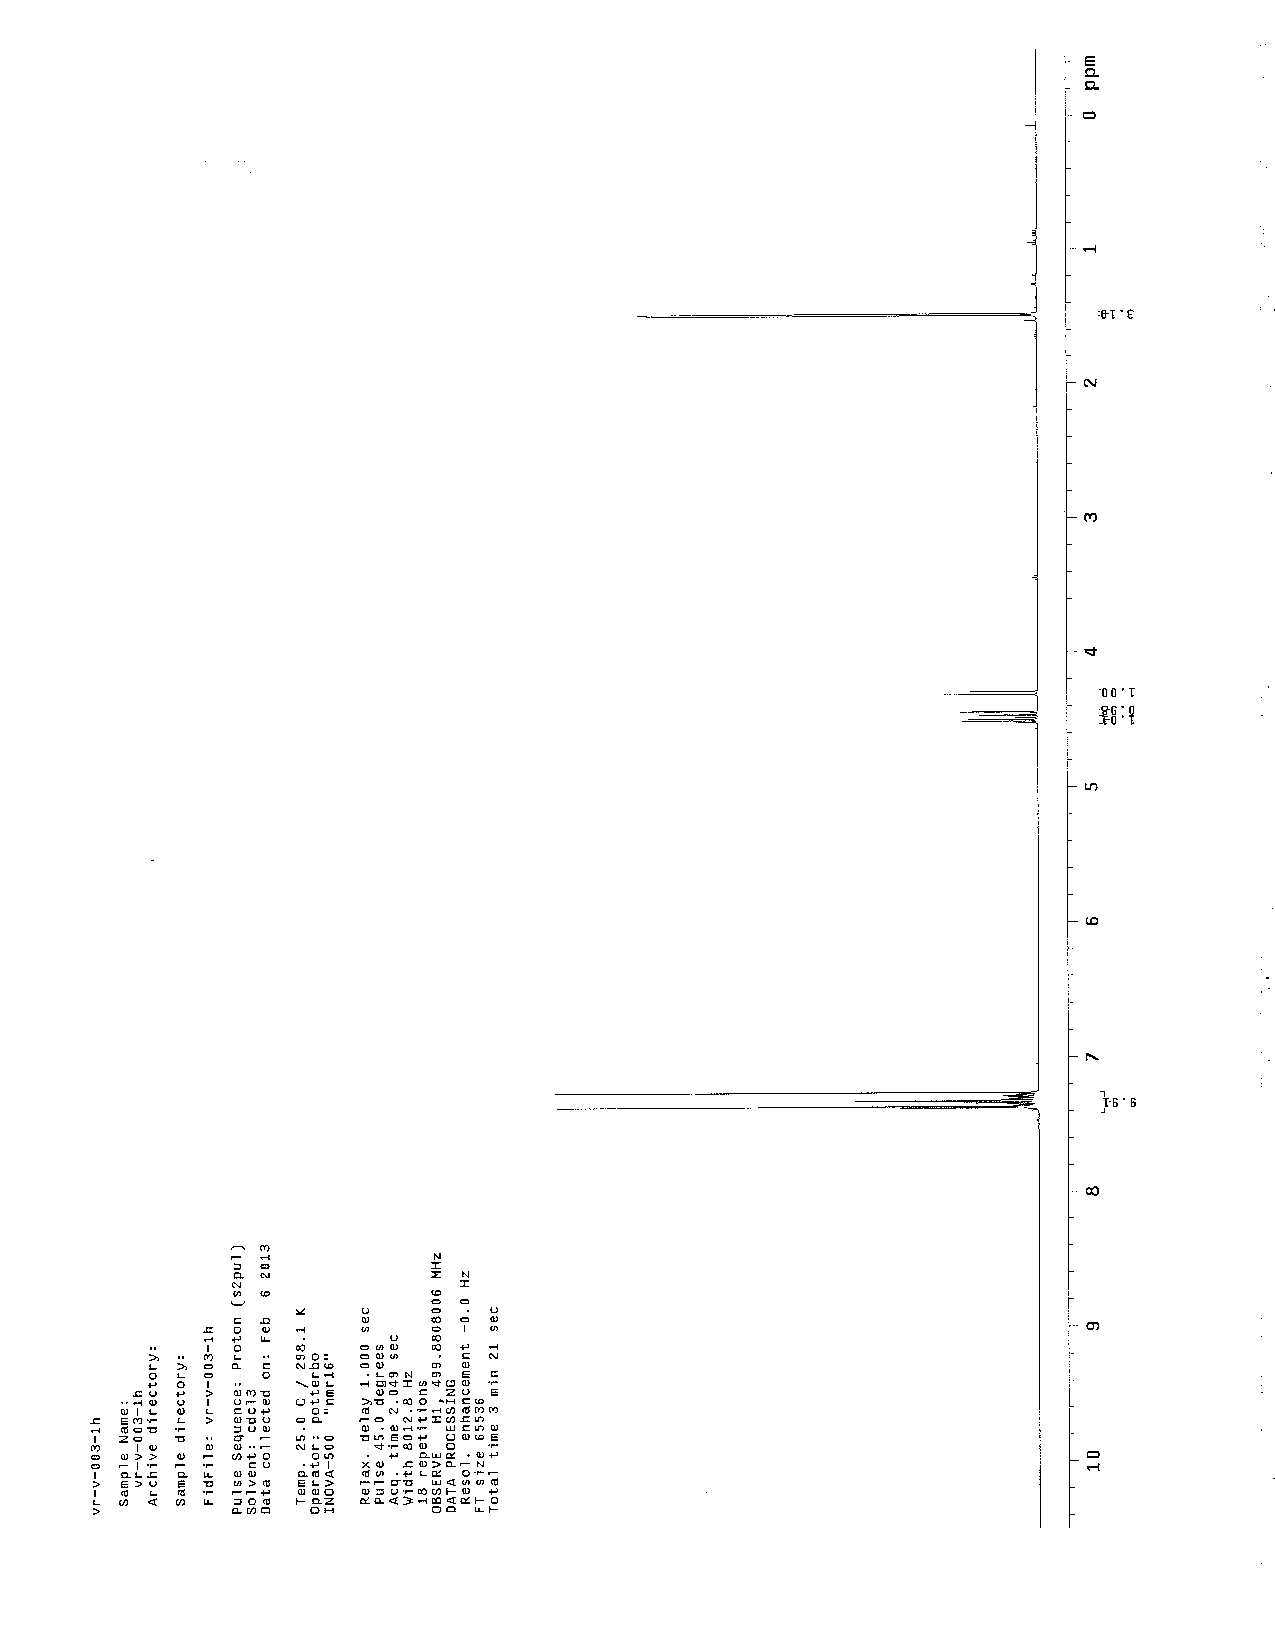
\includegraphics[scale=0.75, trim = 0mm 0mm 0mm 5mm,
clip]{chp_alkylation/images/nmr/xcaaH}
\vspace{-100pt}
\end{figure}
\end{textblock}
\begin{textblock}{1}(2,1)
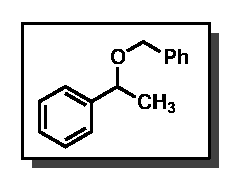
\includegraphics[scale=0.8, angle=90]{chp_alkylation/images/xcaa}
\end{textblock}
\clearpage
%%%
\begin{textblock}{20}(0,0)
\begin{figure}[htb]
\caption{$^{13}$C NMR of  \CMPxcaa\ (\ref{cmp:xcaa})}
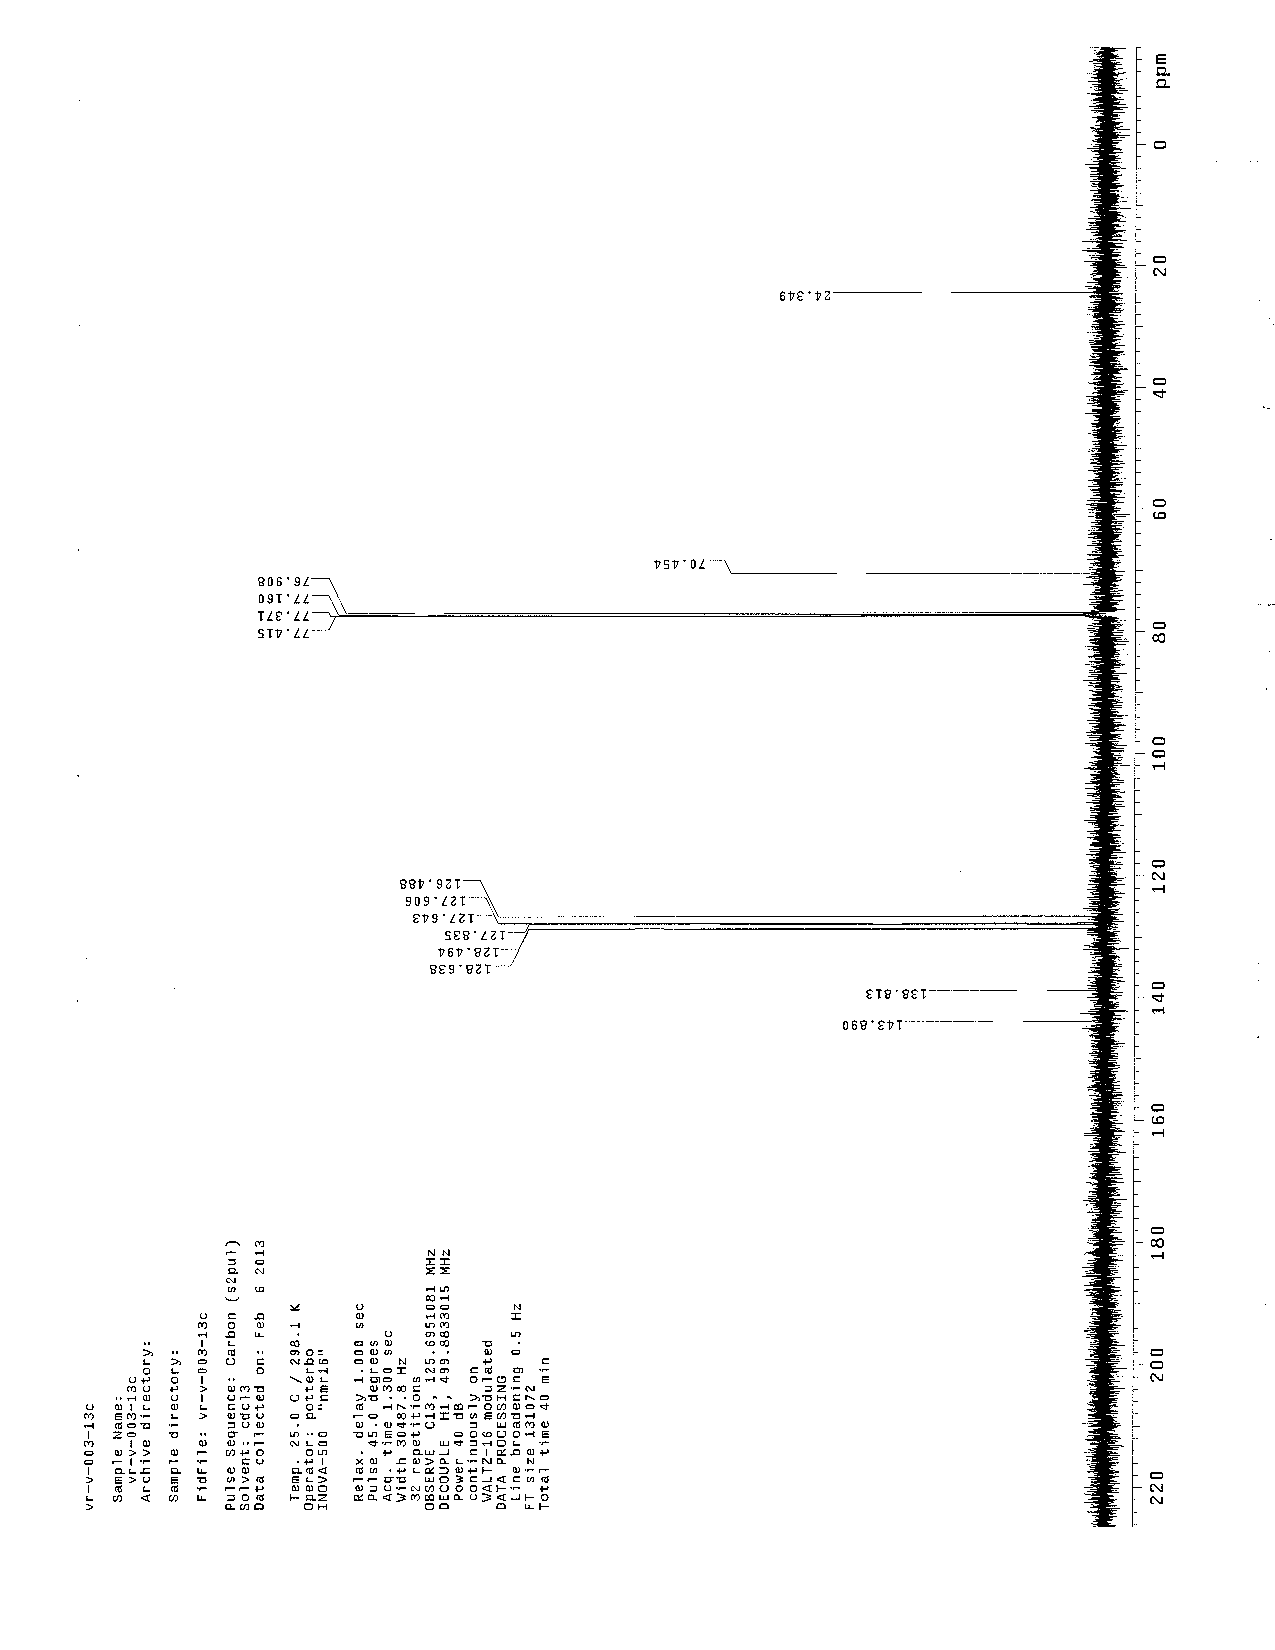
\includegraphics[scale=0.75, trim = 0mm 0mm 0mm 5mm,
clip]{chp_alkylation/images/nmr/xcaaC}
\vspace{-100pt}
\end{figure}
\end{textblock}
\begin{textblock}{1}(2,1)
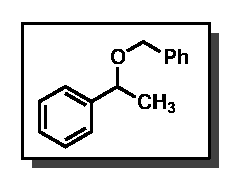
\includegraphics[scale=0.8, angle=90]{chp_alkylation/images/xcaa}
\end{textblock}
\clearpage
%=-=-=-=-=-=-=-=-=-=-=-=-=-=-=-=-=-=-=-=-=-=-=-=-=-=-=-=-=-=-=-=-=-=-=-=-=-=-=-=-=

%=[xcao]=-=-=-=-=-=-=-=-=-=-=-=-=-=-=-=-=-=-=-=-=-=-=-=-=-=-=-=-=-=-=-=-=-=-=-=-=-=-=
\begin{textblock}{20}(0,0)
\begin{figure}[htb]
\caption{$^1$H NMR of \CMPxcao\ (\ref{cmp:xcao})}
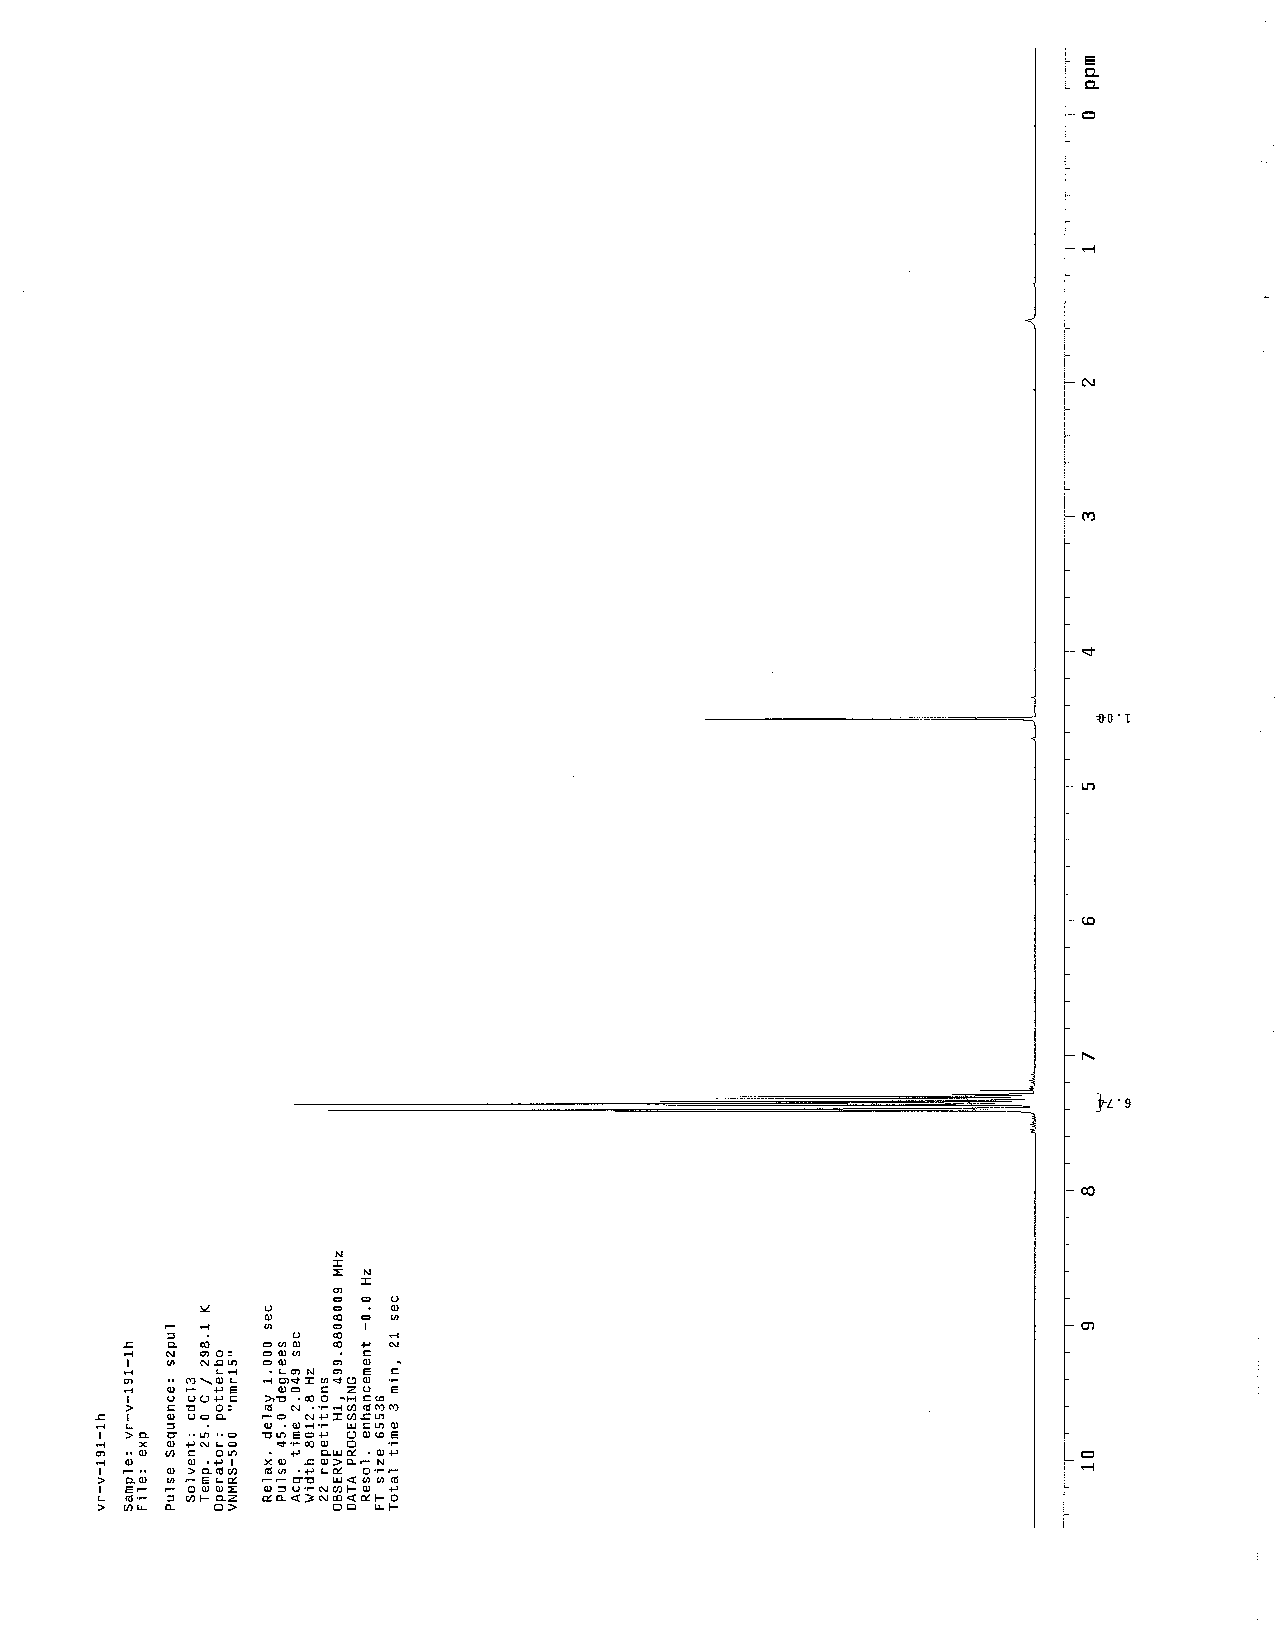
\includegraphics[scale=0.75, trim = 0mm 0mm 0mm 5mm,
clip]{chp_alkylation/images/nmr/xcaoH}
\vspace{-100pt}
\end{figure}
\end{textblock}
\begin{textblock}{1}(2,1)
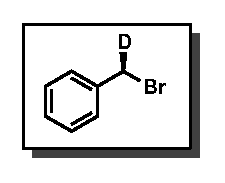
\includegraphics[scale=0.8, angle=90]{chp_alkylation/images/xcao}
\end{textblock}
\clearpage
%%%
\begin{textblock}{20}(0,0)
\begin{figure}[htb]
\caption{$^{13}$C NMR of  \CMPxcao\ (\ref{cmp:xcao})}
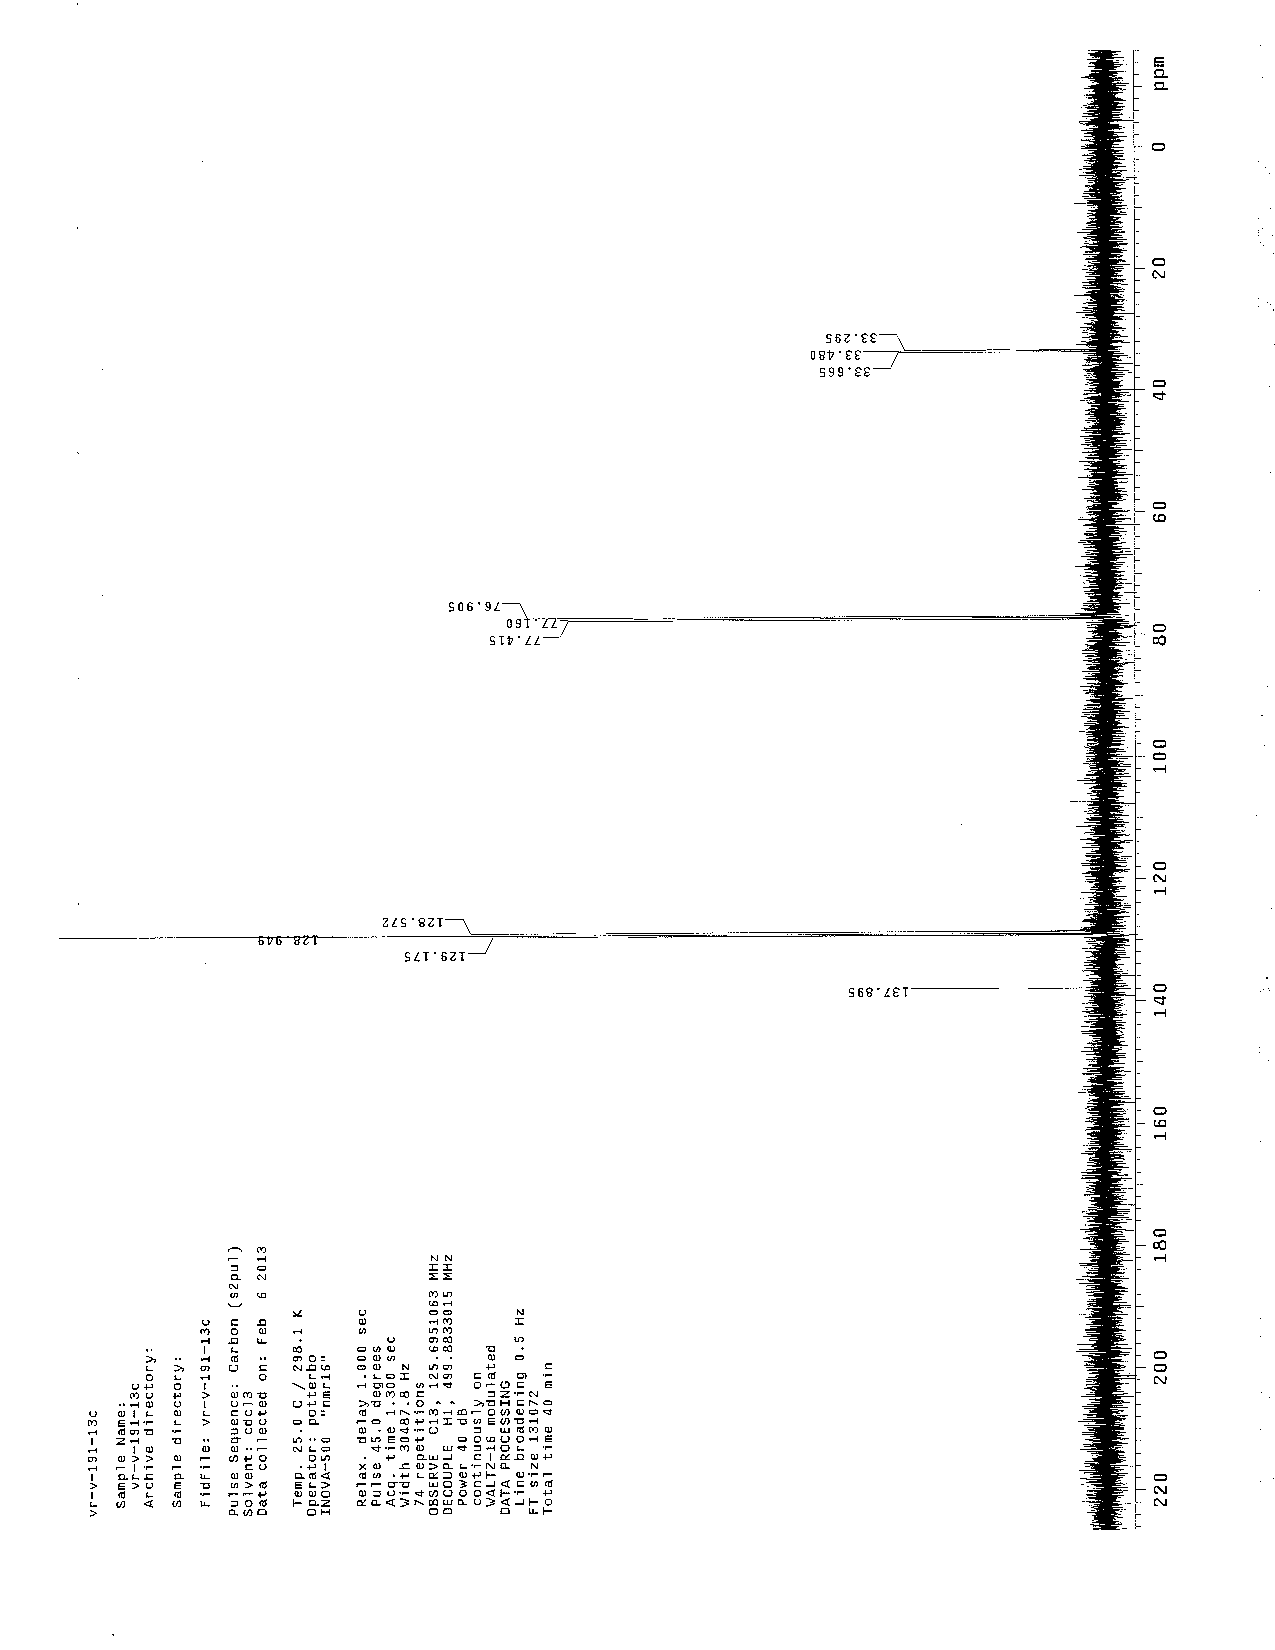
\includegraphics[scale=0.75, trim = 0mm 0mm 0mm 5mm,
clip]{chp_alkylation/images/nmr/xcaoC}
\vspace{-100pt}
\end{figure}
\end{textblock}
\begin{textblock}{1}(2,1)
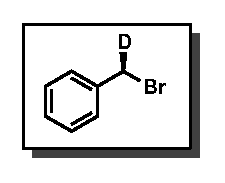
\includegraphics[scale=0.8, angle=90]{chp_alkylation/images/xcao}
\end{textblock}
\clearpage
%=-=-=-=-=-=-=-=-=-=-=-=-=-=-=-=-=-=-=-=-=-=-=-=-=-=-=-=-=-=-=-=-=-=-=-=-=-=-=-=-=

%=[xcab]=-=-=-=-=-=-=-=-=-=-=-=-=-=-=-=-=-=-=-=-=-=-=-=-=-=-=-=-=-=-=-=-=-=-=-=-=-=-=
\begin{textblock}{20}(0,0)
\begin{figure}[htb]
\caption{$^1$H NMR of \CMPxcab\ (\ref{cmp:xcab})}
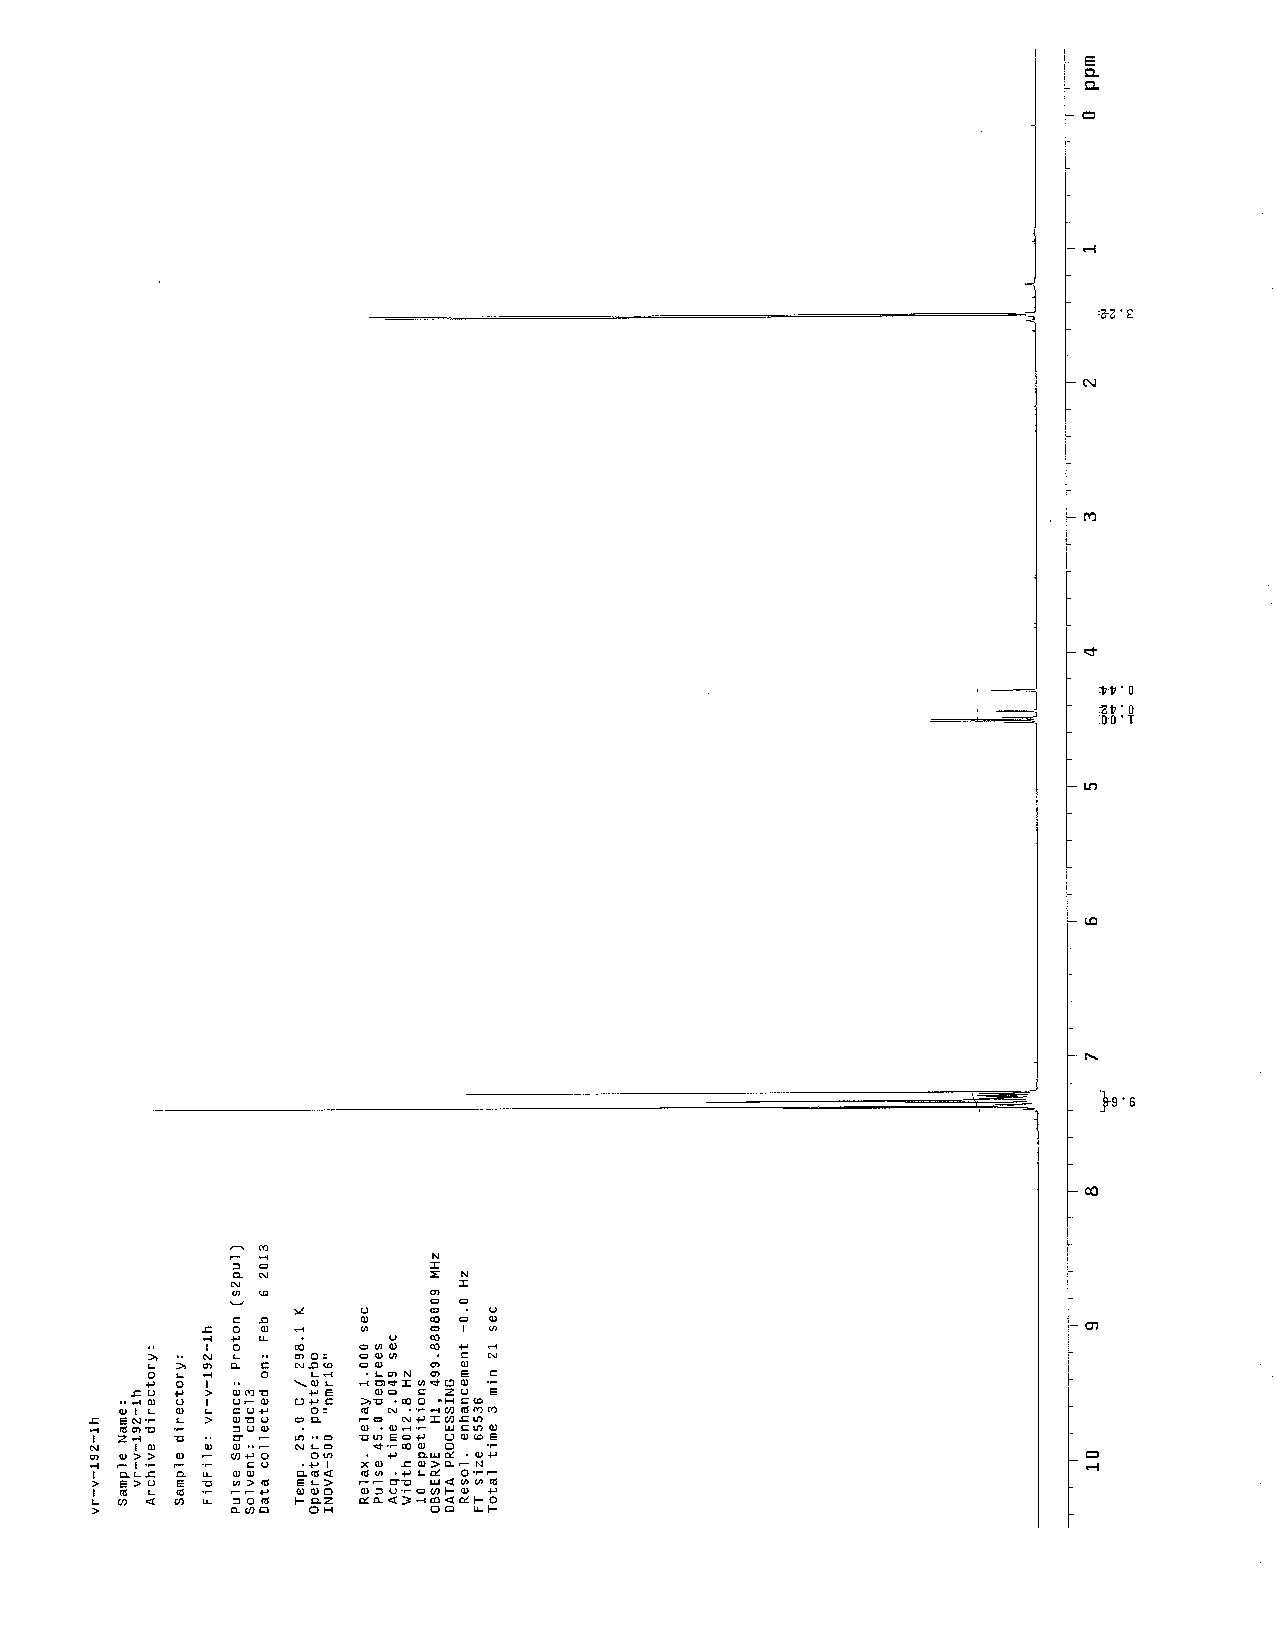
\includegraphics[scale=0.75, trim = 0mm 0mm 0mm 5mm,
clip]{chp_alkylation/images/nmr/xcabH}
\vspace{-100pt}
\end{figure}
\end{textblock}
\begin{textblock}{1}(2,1)
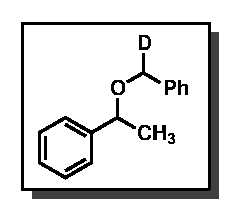
\includegraphics[scale=0.8, angle=90]{chp_alkylation/images/xcab}
\end{textblock}
\clearpage
%%%
\begin{textblock}{20}(0,0)
\begin{figure}[htb]
\caption{$^{13}$C NMR of  \CMPxcab\ (\ref{cmp:xcab})}
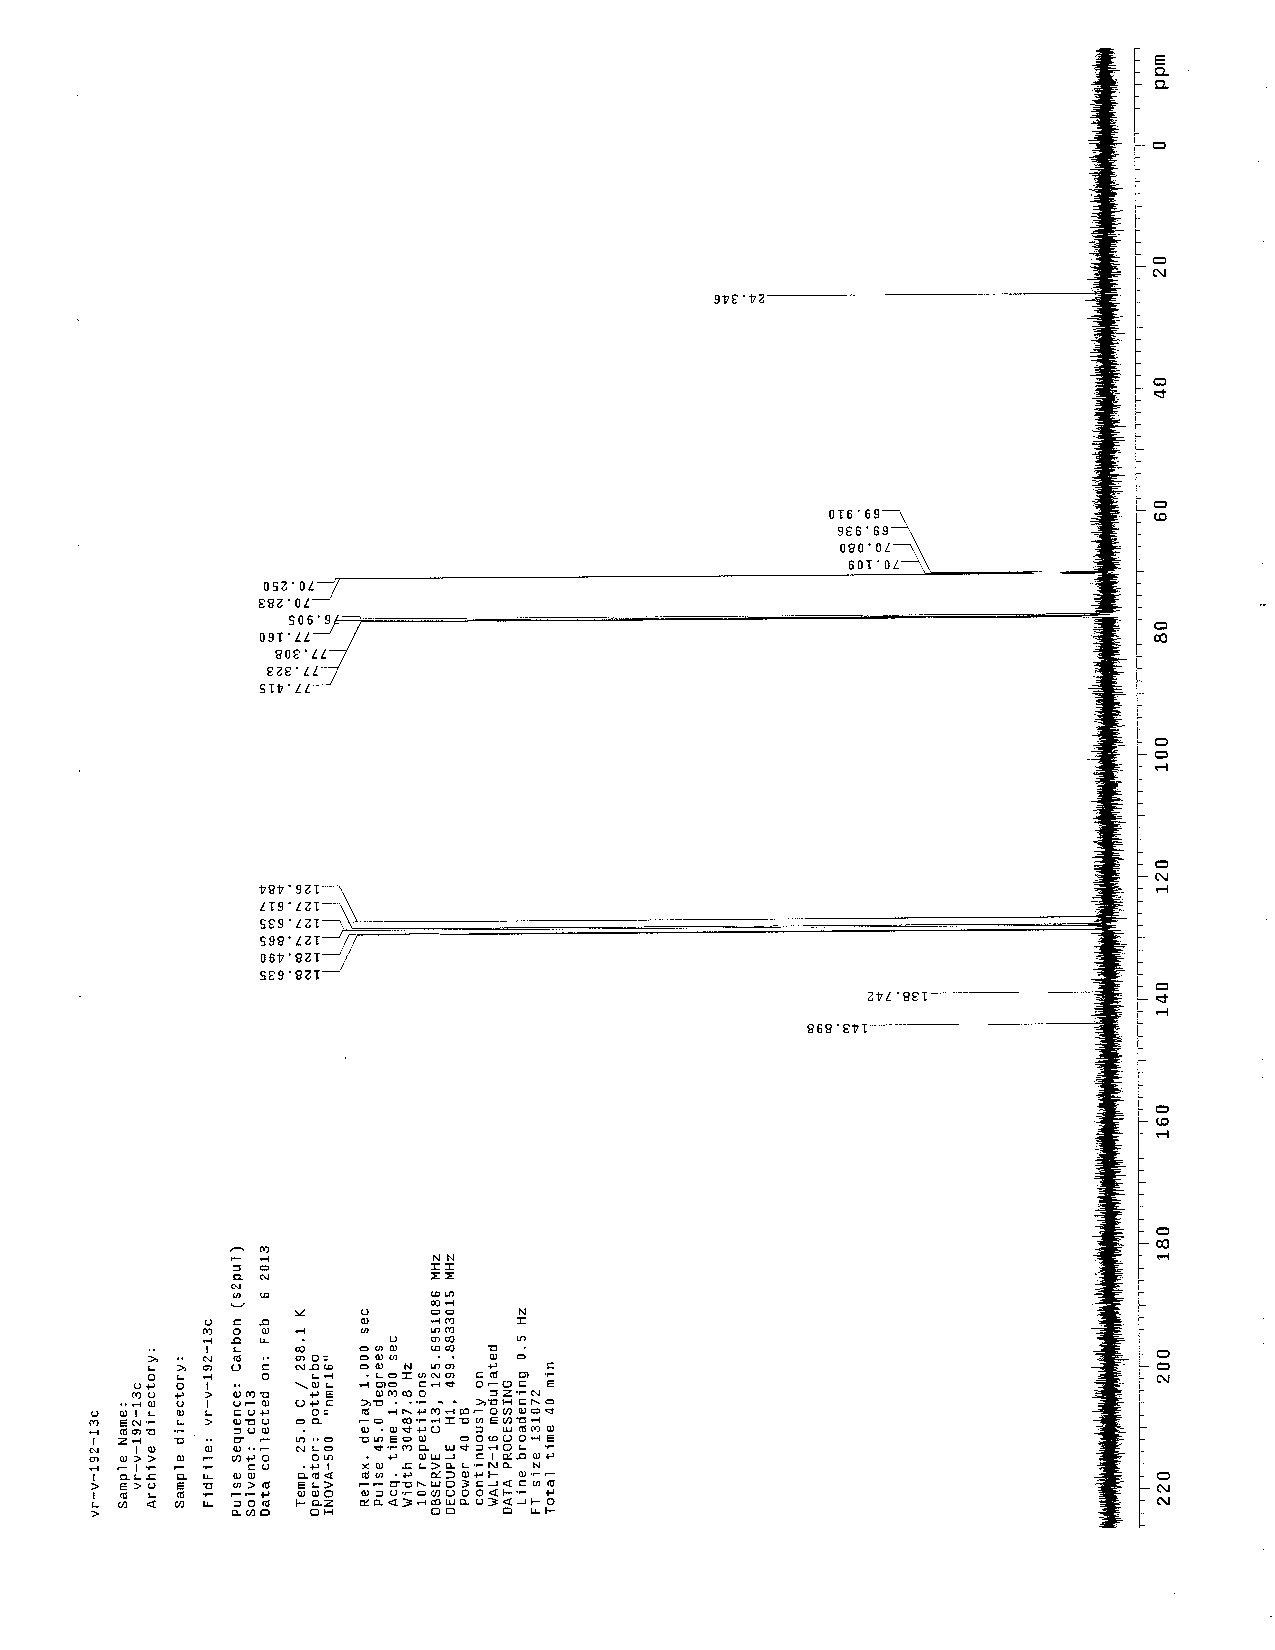
\includegraphics[scale=0.75, trim = 0mm 0mm 0mm 5mm,
clip]{chp_alkylation/images/nmr/xcabC}
\vspace{-100pt}
\end{figure}
\end{textblock}
\begin{textblock}{1}(2,1)
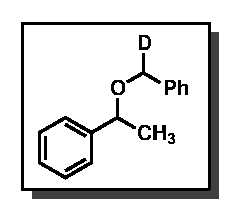
\includegraphics[scale=0.8, angle=90]{chp_alkylation/images/xcab}
\end{textblock}
\clearpage
%=-=-=-=-=-=-=-=-=-=-=-=-=-=-=-=-=-=-=-=-=-=-=-=-=-=-=-=-=-=-=-=-=-=-=-=-=-=-=-=-=

%=[xcac]=-=-=-=-=-=-=-=-=-=-=-=-=-=-=-=-=-=-=-=-=-=-=-=-=-=-=-=-=-=-=-=-=-=-=-=-=-=-=
\begin{textblock}{20}(0,0)
\begin{figure}[htb]
\caption{$^1$H NMR of \CMPxcac\ (\ref{cmp:xcac})}
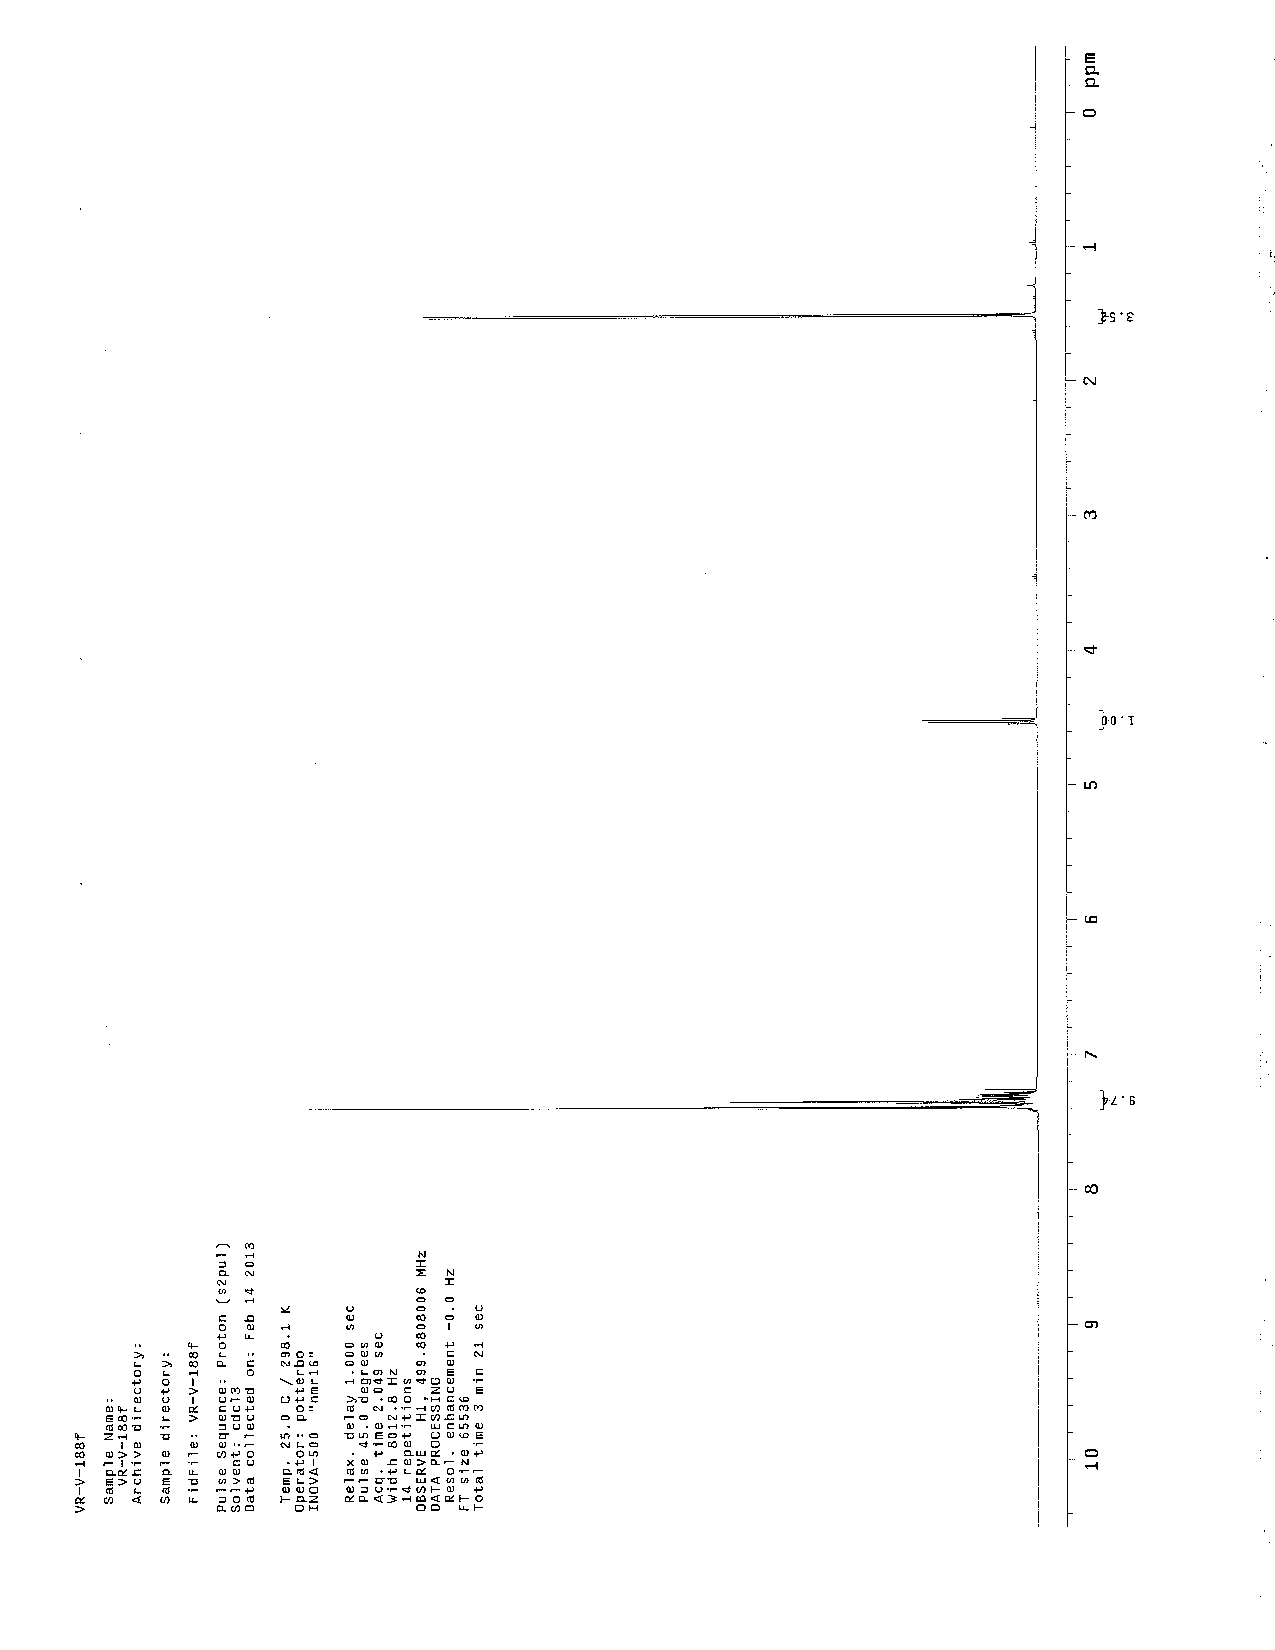
\includegraphics[scale=0.75, trim = 0mm 0mm 0mm 5mm,
clip]{chp_alkylation/images/nmr/xcacH}
\vspace{-100pt}
\end{figure}
\end{textblock}
\begin{textblock}{1}(2,1)
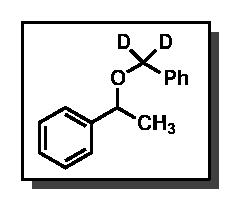
\includegraphics[scale=0.8, angle=90]{chp_alkylation/images/xcac}
\end{textblock}
\clearpage
%%%
\begin{textblock}{20}(0,0)
\begin{figure}[htb]
\caption{$^{13}$C NMR of  \CMPxcac\ (\ref{cmp:xcac})}
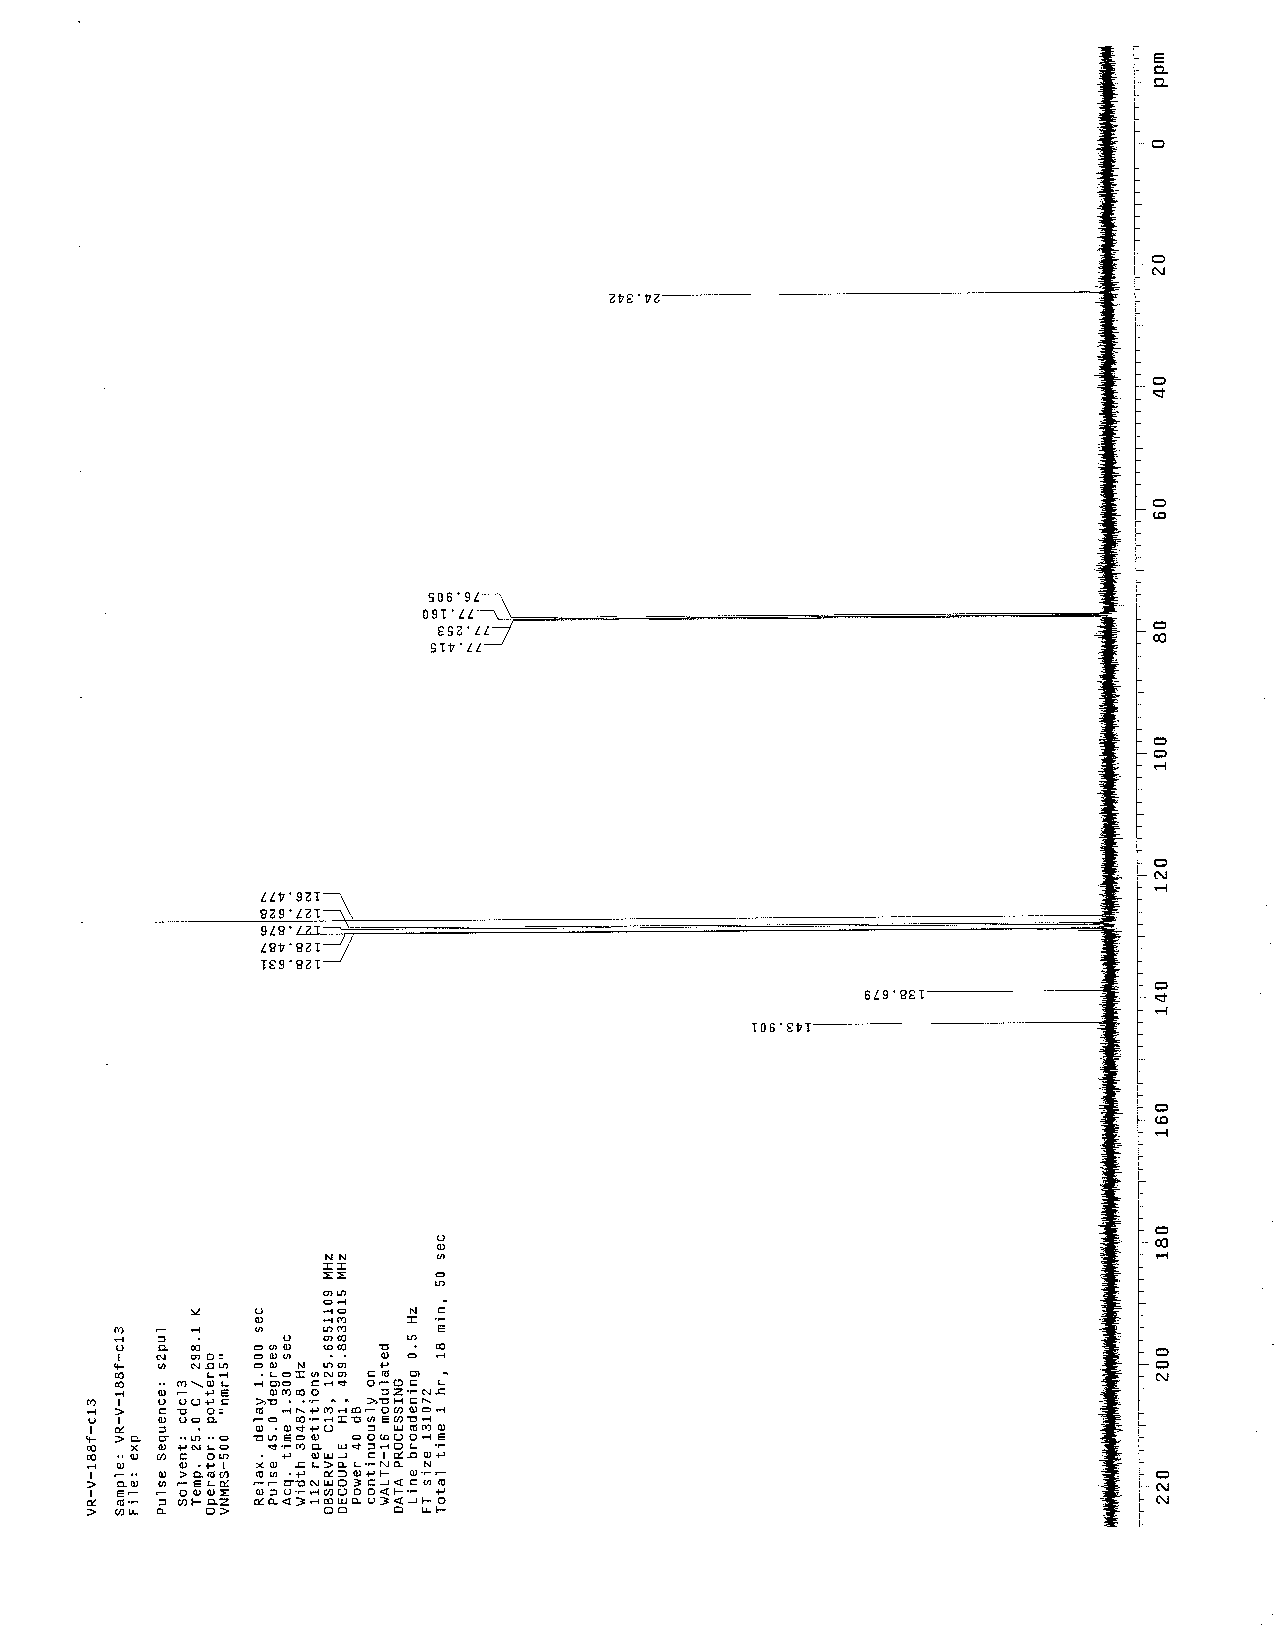
\includegraphics[scale=0.75, trim = 0mm 0mm 0mm 5mm,
clip]{chp_alkylation/images/nmr/xcacC}
\vspace{-100pt}
\end{figure}
\end{textblock}
\begin{textblock}{1}(2,1)
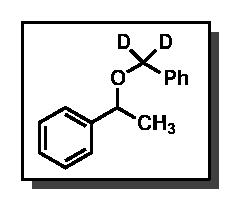
\includegraphics[scale=0.8, angle=90]{chp_alkylation/images/xcac}
\end{textblock}
\clearpage
%=-=-=-=-=-=-=-=-=-=-=-=-=-=-=-=-=-=-=-=-=-=-=-=-=-=-=-=-=-=-=-=-=-=-=-=-=-=-=-=-=

%=[xcad]=-=-=-=-=-=-=-=-=-=-=-=-=-=-=-=-=-=-=-=-=-=-=-=-=-=-=-=-=-=-=-=-=-=-=-=-=-=-=
\begin{textblock}{20}(0,0)
\begin{figure}[htb]
\caption{$^1$H NMR of \CMPxcad\ (\ref{cmp:xcad})}
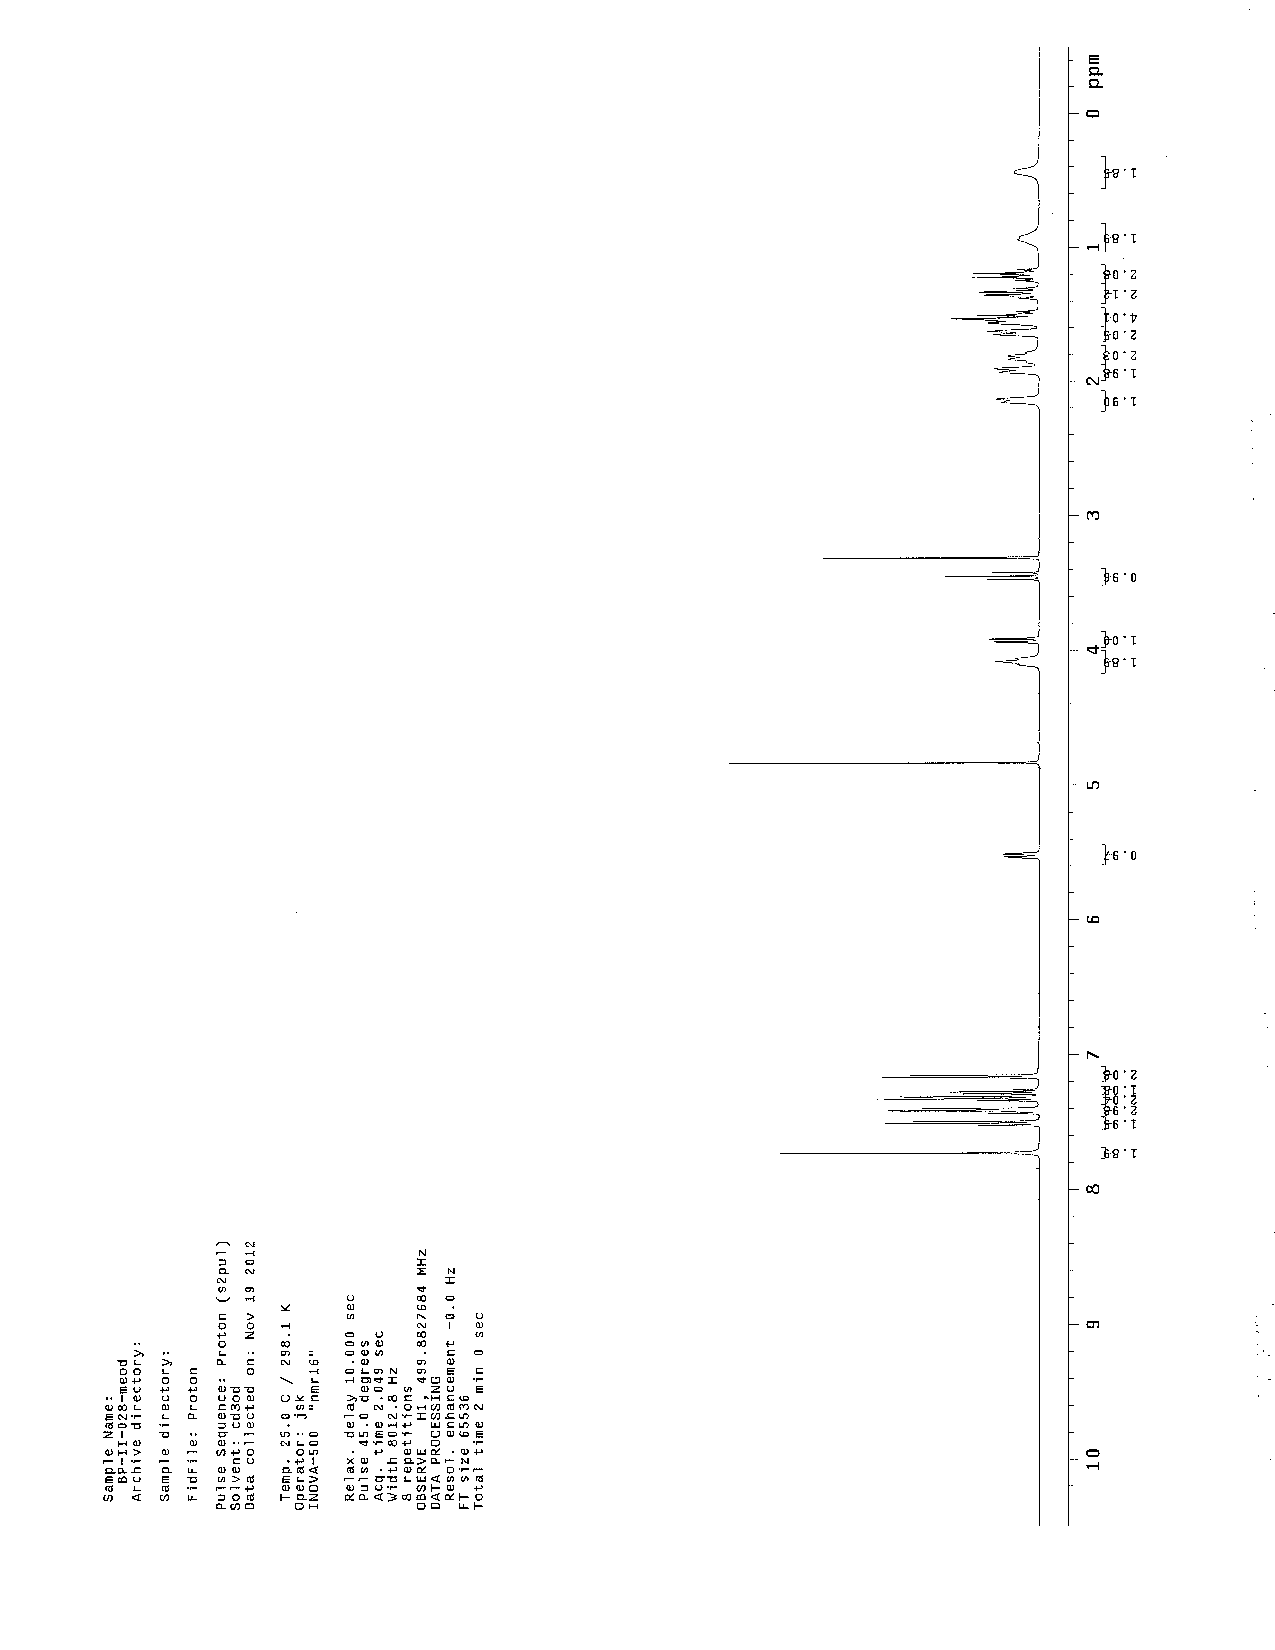
\includegraphics[scale=0.75, trim = 0mm 0mm 0mm 5mm,
clip]{chp_alkylation/images/nmr/xcadH}
\vspace{-100pt}
\end{figure}
\end{textblock}
\begin{textblock}{1}(2,1)
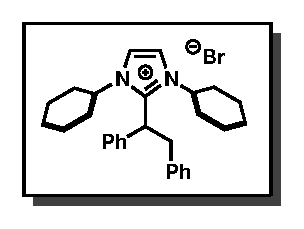
\includegraphics[scale=0.8, angle=90]{chp_alkylation/images/xcad}
\end{textblock}
\clearpage
%%%
\begin{textblock}{20}(0,0)
\begin{figure}[htb]
\caption{$^{13}$C NMR of  \CMPxcad\ (\ref{cmp:xcad})}
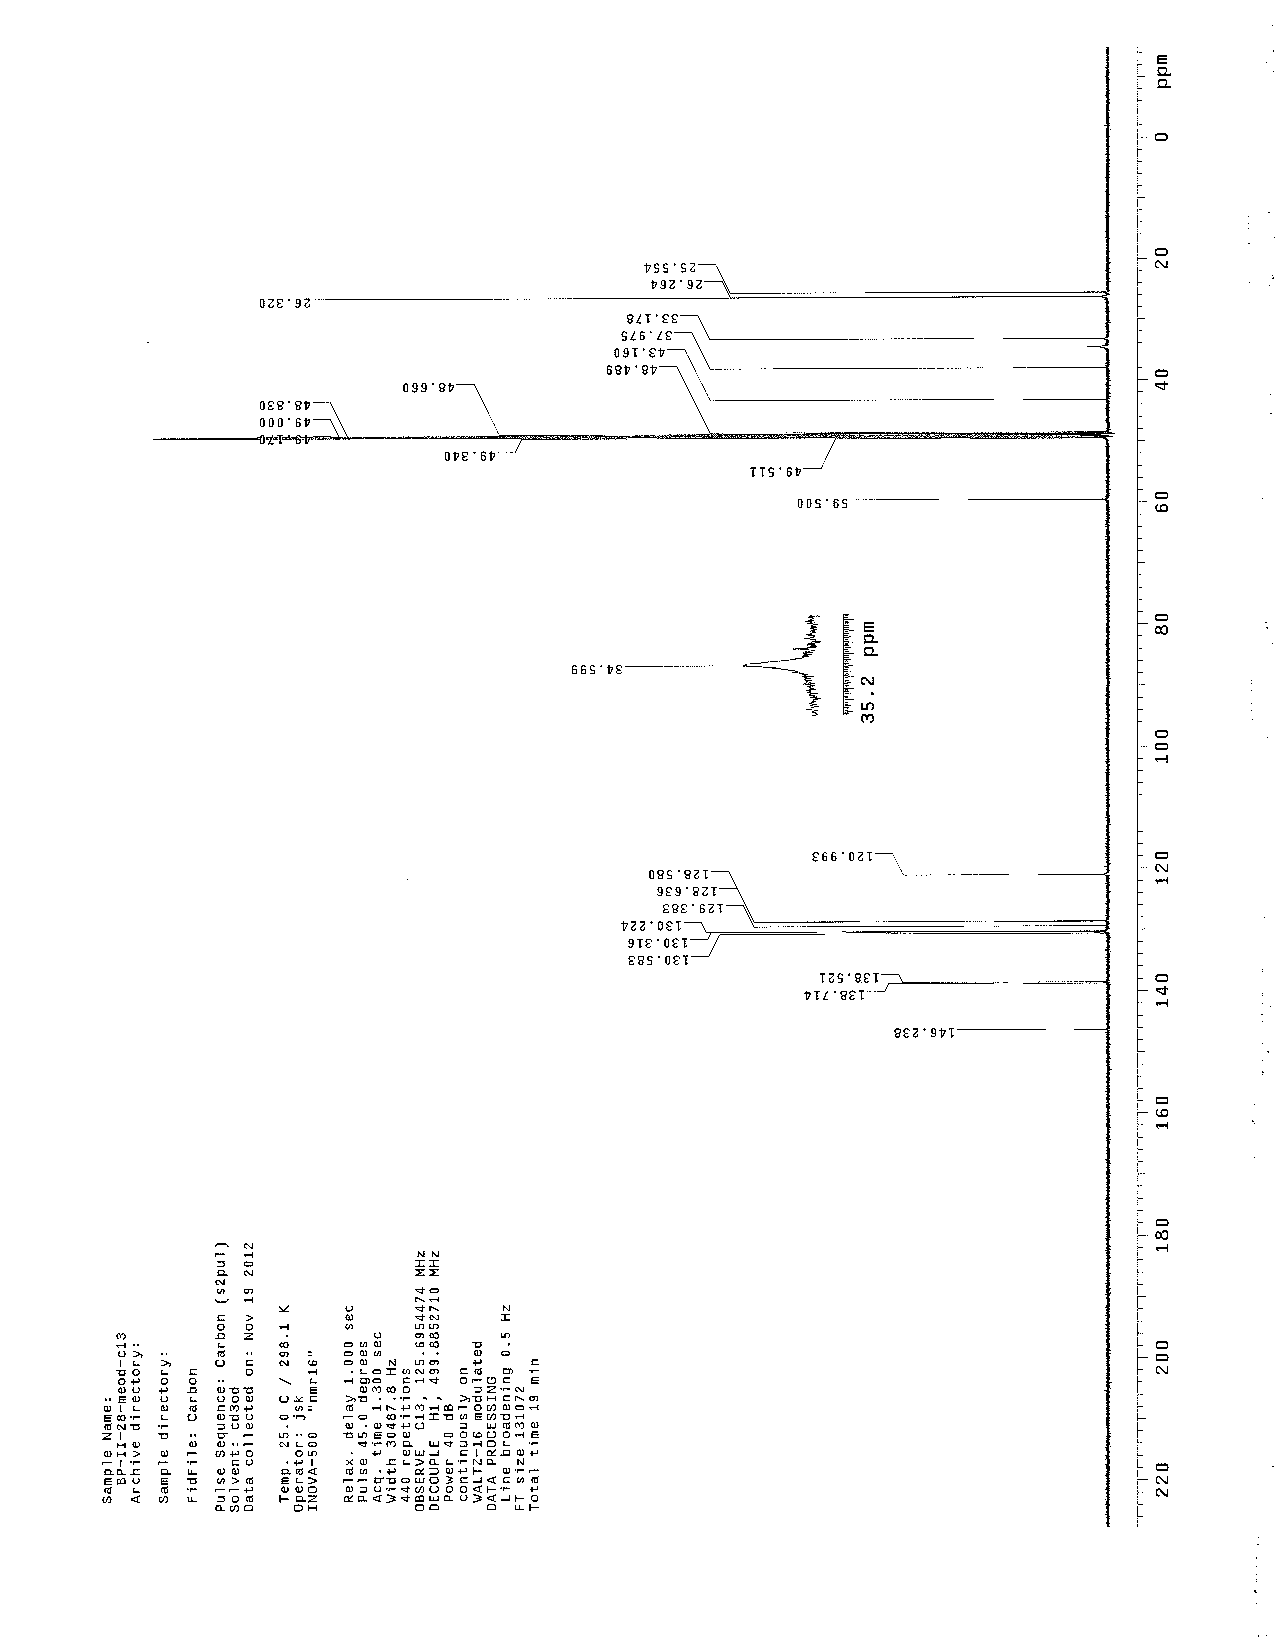
\includegraphics[scale=0.75, trim = 0mm 0mm 0mm 5mm,
clip]{chp_alkylation/images/nmr/xcadC}
\vspace{-100pt}
\end{figure}
\end{textblock}
\begin{textblock}{1}(2,10)
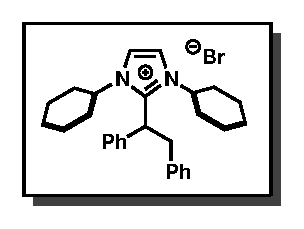
\includegraphics[scale=0.8, angle=90]{chp_alkylation/images/xcad}
\end{textblock}
\clearpage
%%%
\begin{textblock}{20}(0,0)
\begin{figure}[htb]
\caption{HSQC NMR of  \CMPxcad\ (\ref{cmp:xcad})}
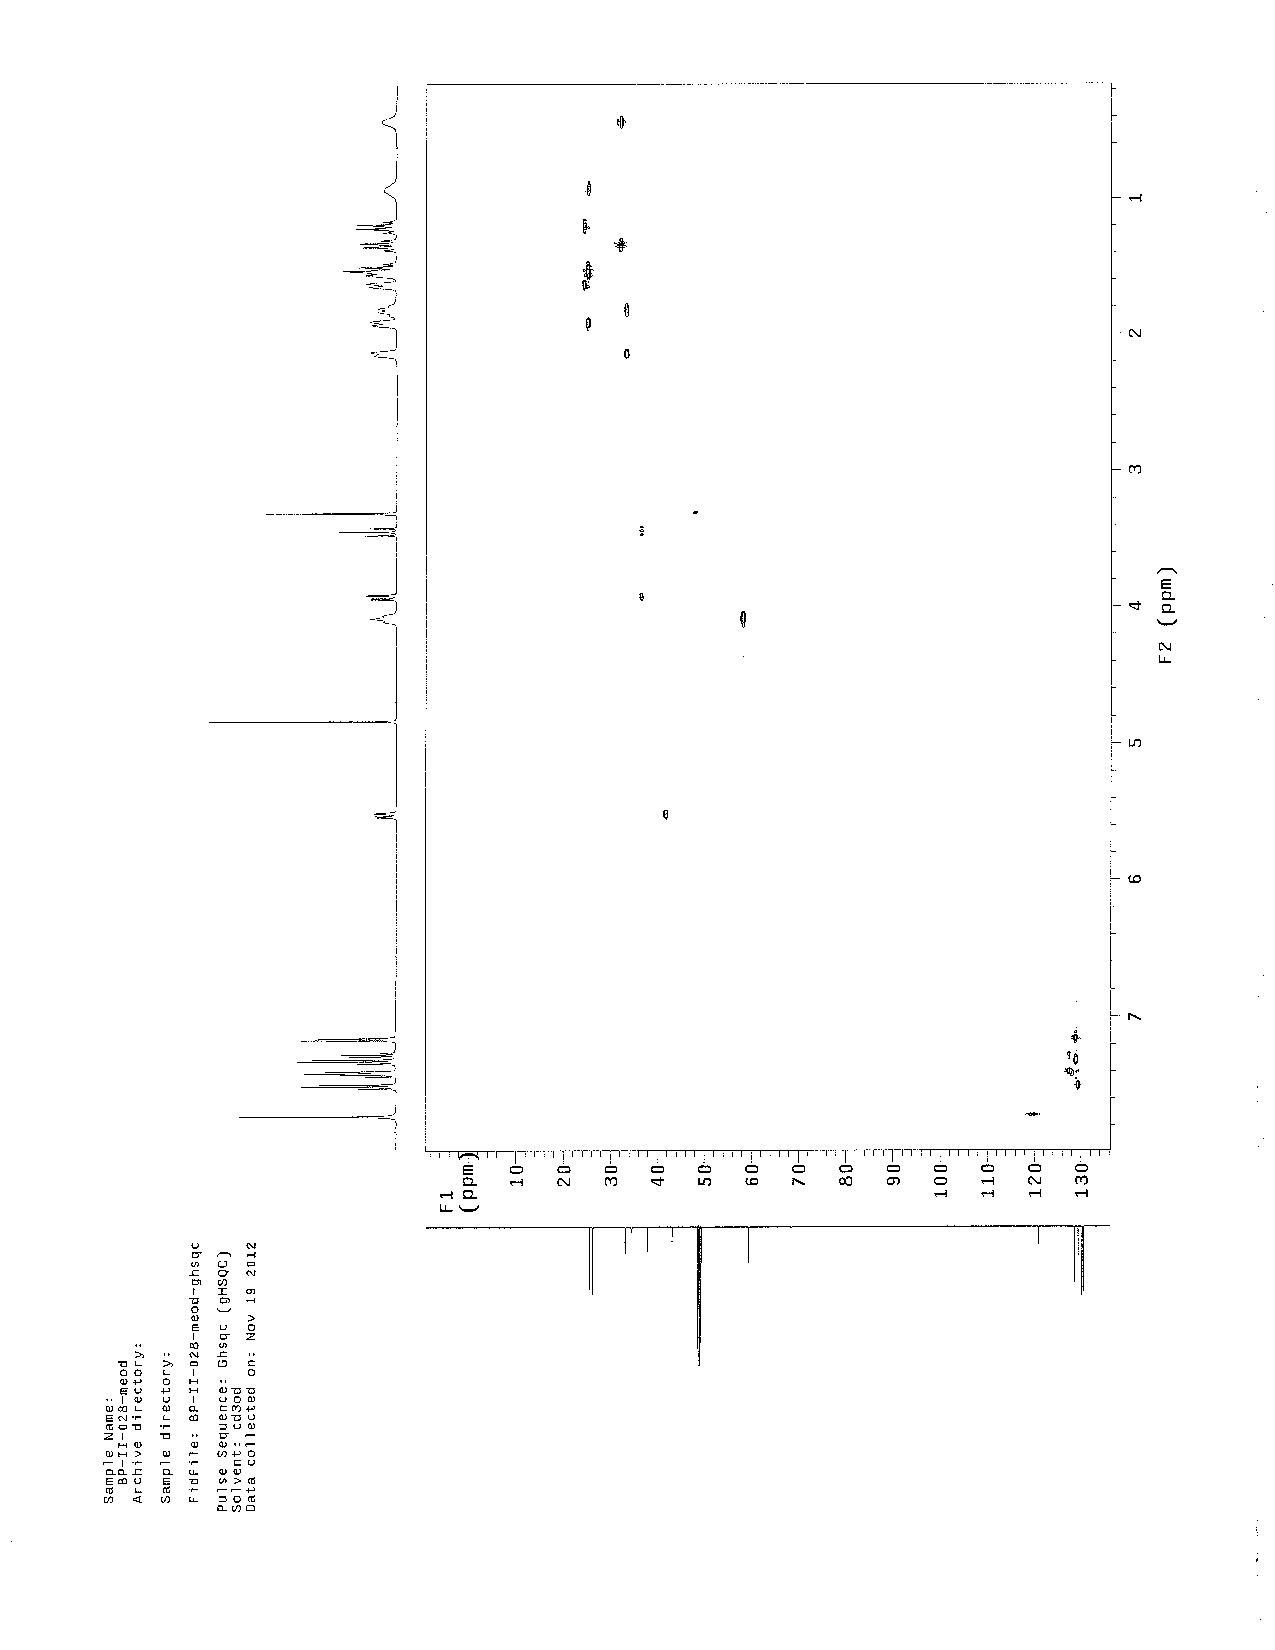
\includegraphics[scale=0.75, trim = 0mm 0mm 0mm 5mm,
clip]{chp_alkylation/images/nmr/xcadHSQC}
\vspace{-100pt}
\end{figure}
\end{textblock}
\begin{textblock}{1}(1,1)
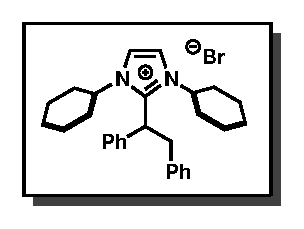
\includegraphics[scale=0.8, angle=90]{chp_alkylation/images/xcad}
\end{textblock}
\clearpage
%=-=-=-=-=-=-=-=-=-=-=-=-=-=-=-=-=-=-=-=-=-=-=-=-=-=-=-=-=-=-=-=-=-=-=-=-=-=-=-=-=

%=[xcae]=-=-=-=-=-=-=-=-=-=-=-=-=-=-=-=-=-=-=-=-=-=-=-=-=-=-=-=-=-=-=-=-=-=-=-=-=-=-=
\begin{textblock}{20}(0,0)
\begin{figure}[htb]
\caption{$^1$H NMR of \CMPxcae\ (\ref{cmp:xcae})}
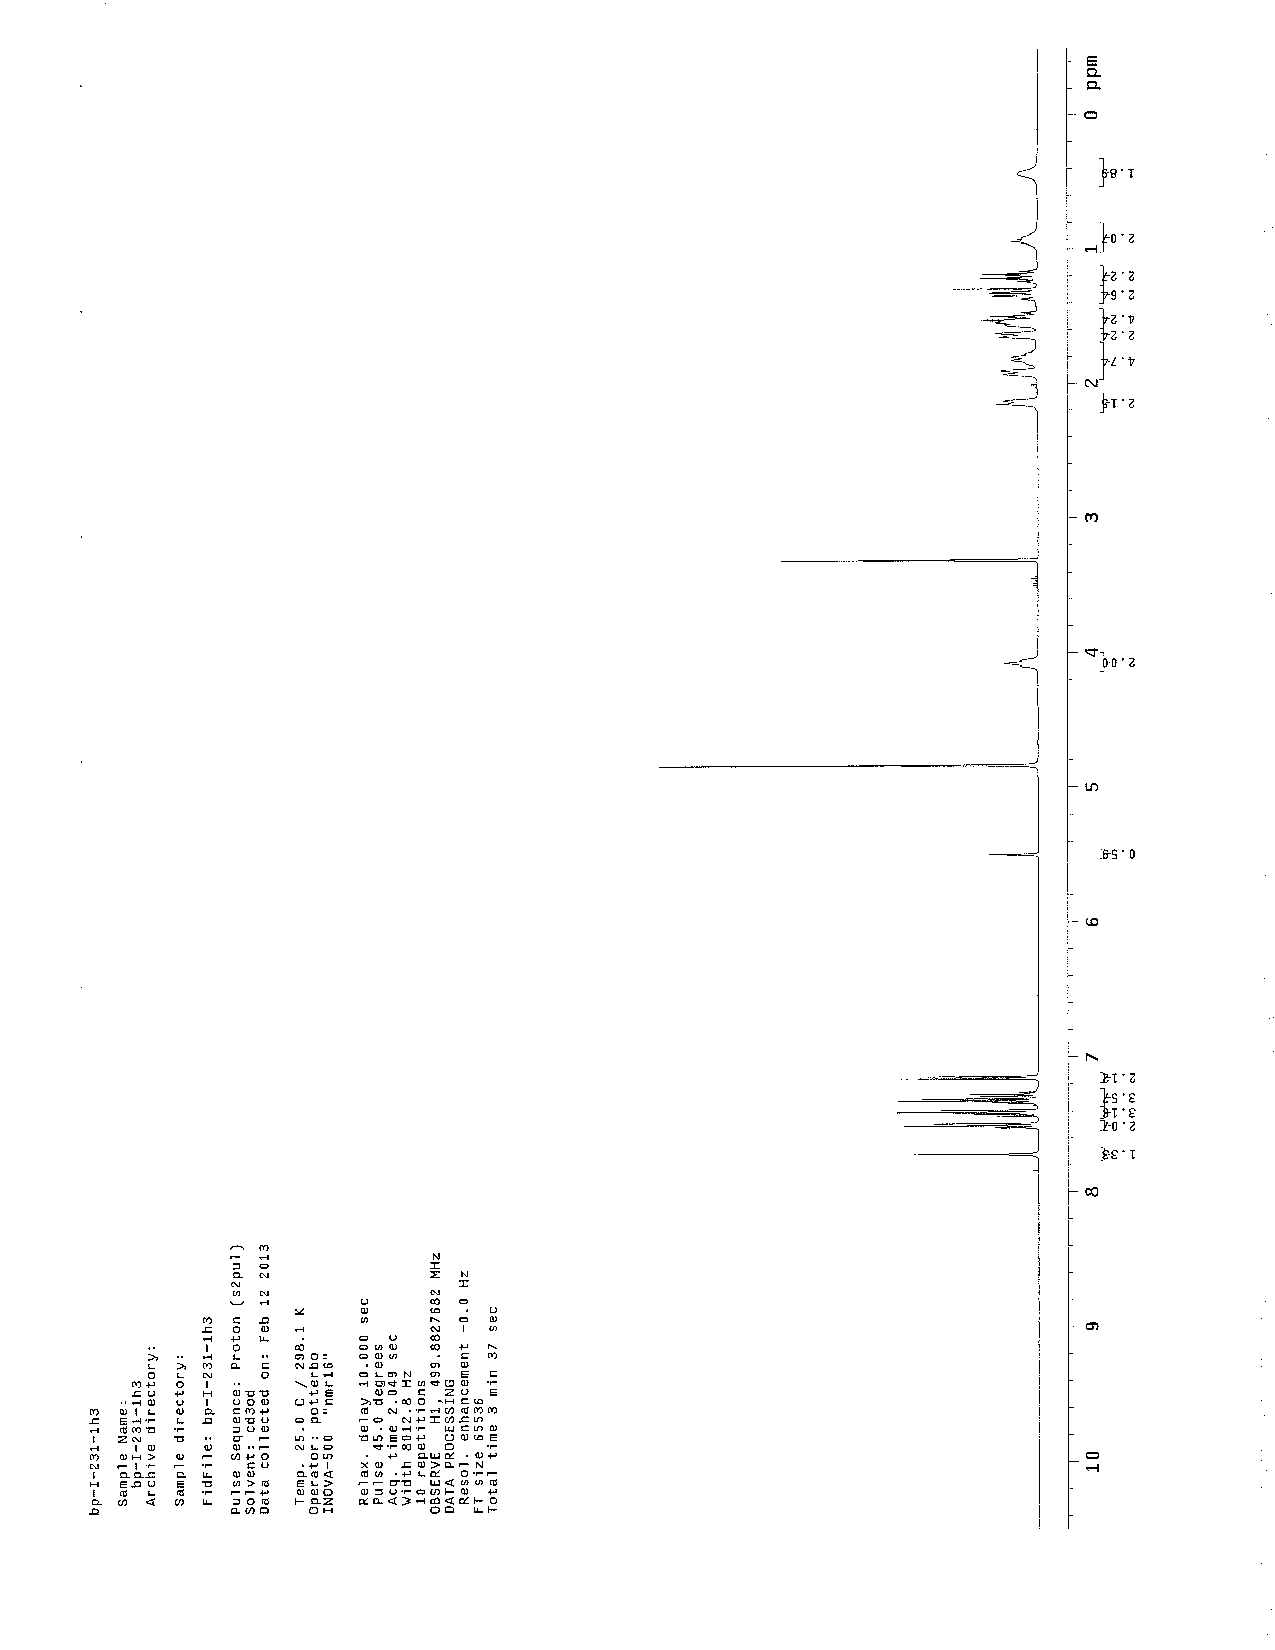
\includegraphics[scale=0.75, trim = 0mm 0mm 0mm 5mm,
clip]{chp_alkylation/images/nmr/xcaeH}
\vspace{-100pt}
\end{figure}
\end{textblock}
\begin{textblock}{1}(2,1)
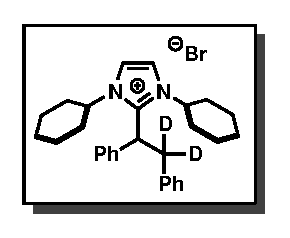
\includegraphics[scale=0.8, angle=90]{chp_alkylation/images/xcae}
\end{textblock}
\clearpage
%%%
\begin{textblock}{20}(0,0)
\begin{figure}[htb]
\caption{$^{13}$C NMR of  \CMPxcae\ (\ref{cmp:xcae})}
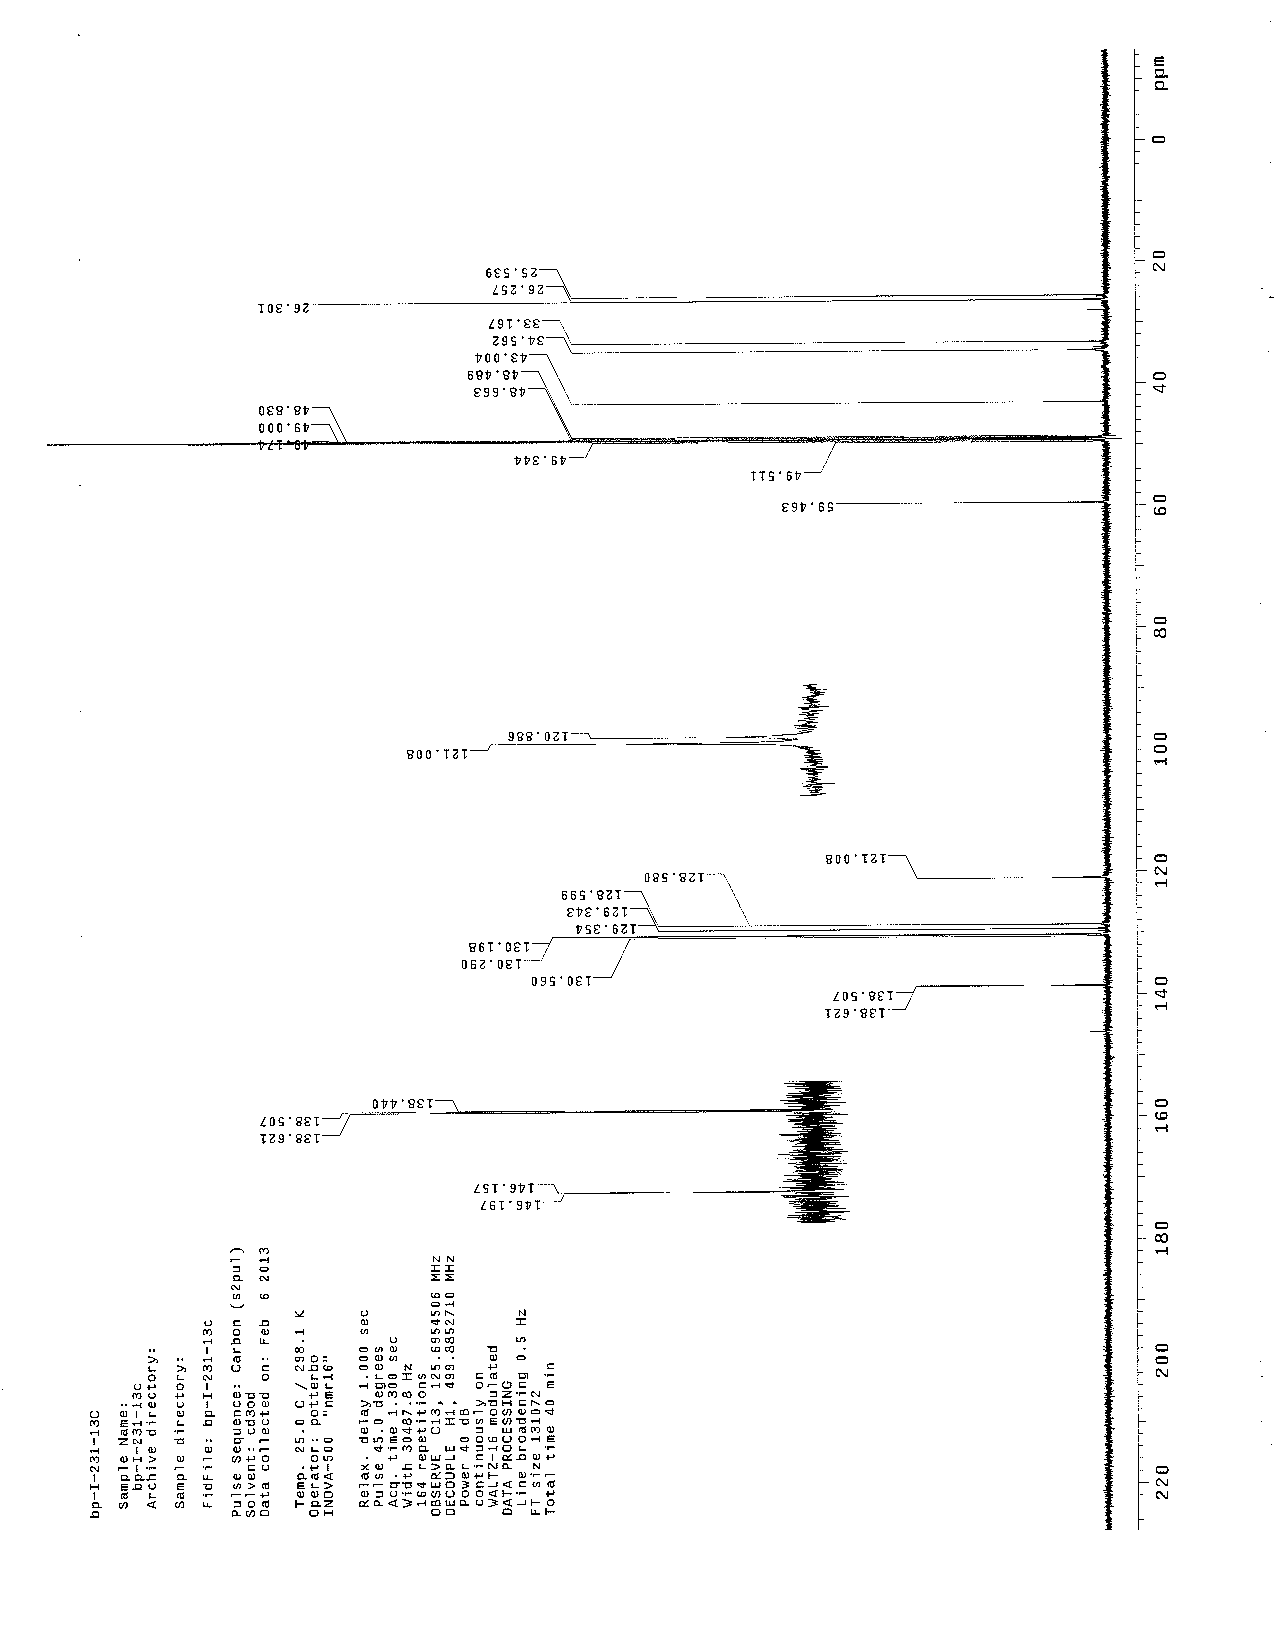
\includegraphics[scale=0.75, trim = 0mm 0mm 0mm 5mm,
clip]{chp_alkylation/images/nmr/xcaeC}
\vspace{-100pt}
\end{figure}
\end{textblock}
\begin{textblock}{1}(2,9)
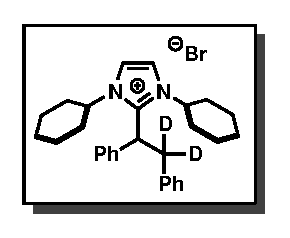
\includegraphics[scale=0.8, angle=90]{chp_alkylation/images/xcae}
\end{textblock}
\clearpage
%=-=-=-=-=-=-=-=-=-=-=-=-=-=-=-=-=-=-=-=-=-=-=-=-=-=-=-=-=-=-=-=-=-=-=-=-=-=-=-=-=

%=[xcaf]=-=-=-=-=-=-=-=-=-=-=-=-=-=-=-=-=-=-=-=-=-=-=-=-=-=-=-=-=-=-=-=-=-=-=-=-=-=-=
\begin{textblock}{20}(0,0)
\begin{figure}[htb]
\caption{$^1$H NMR of \CMPxcaf\ (\ref{cmp:xcaf})}
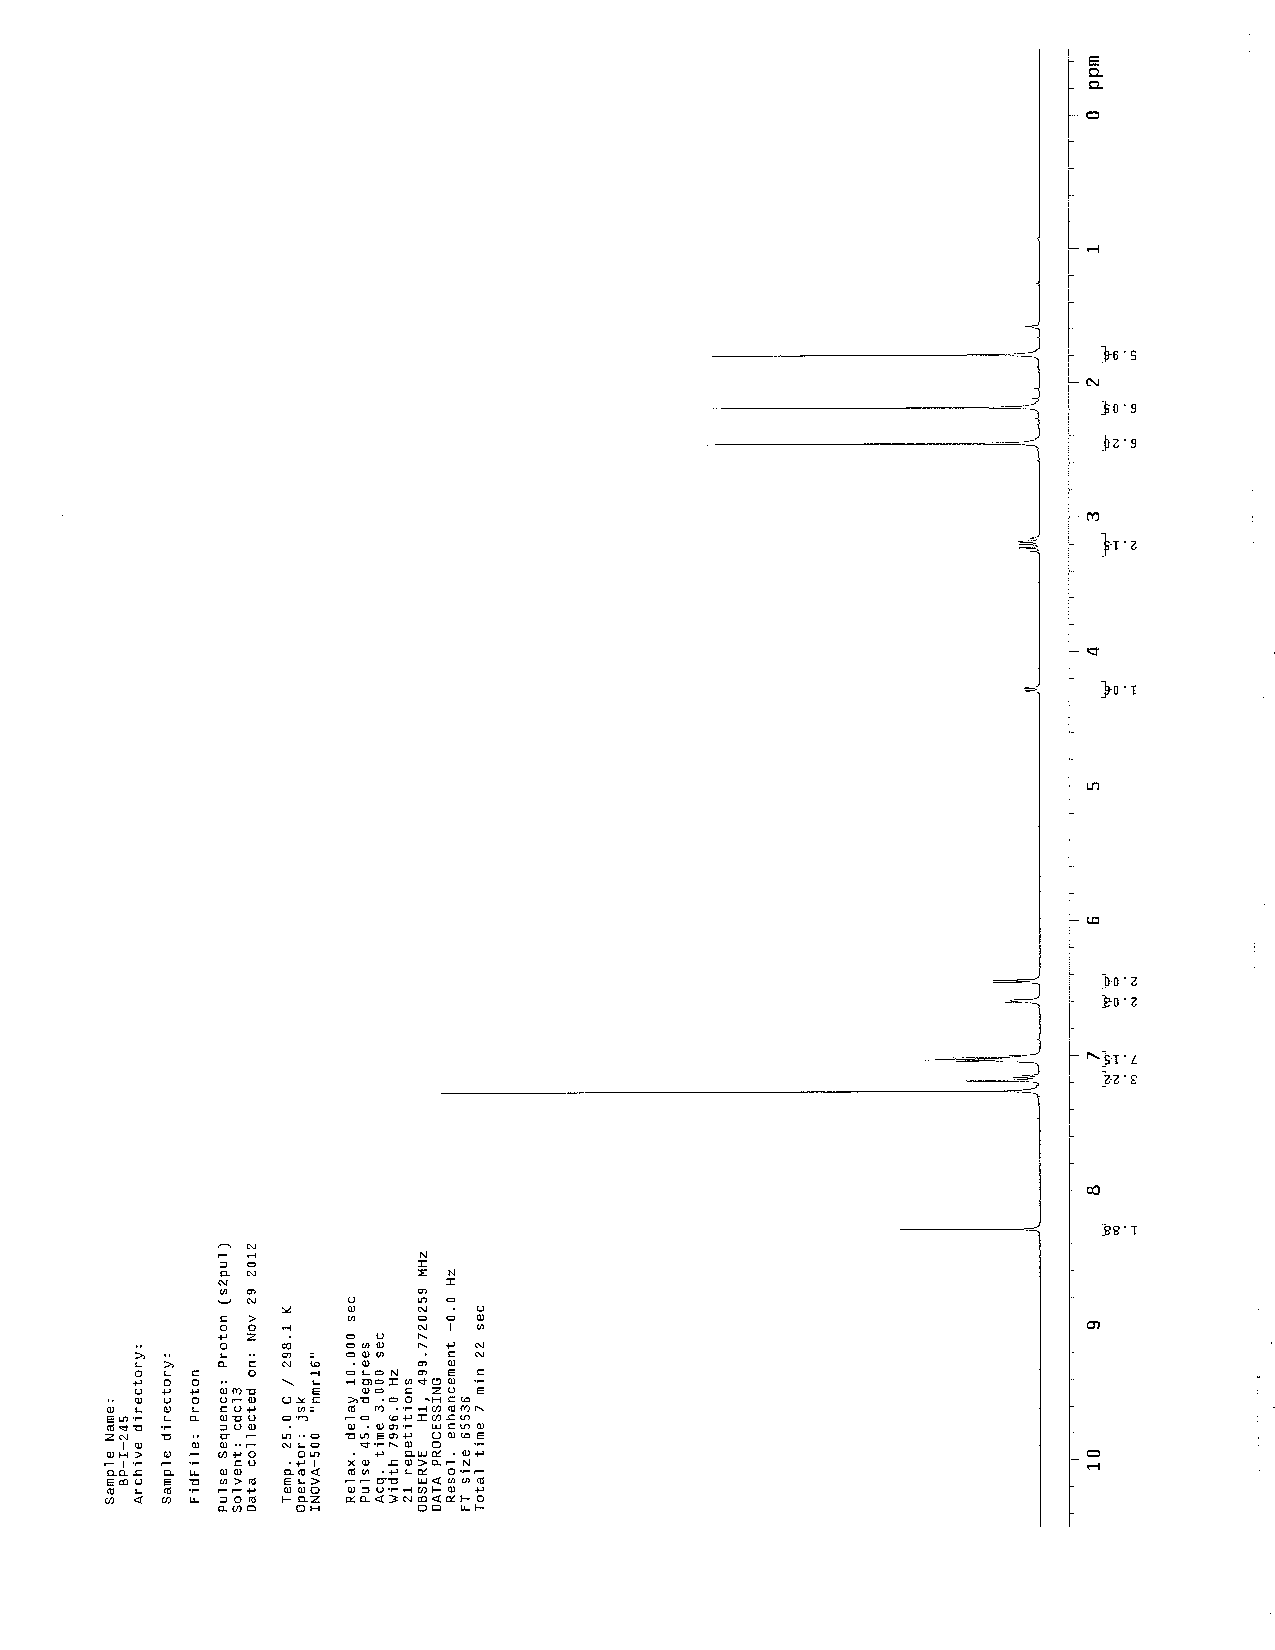
\includegraphics[scale=0.75, trim = 0mm 0mm 0mm 5mm,
clip]{chp_alkylation/images/nmr/xcafH}
\vspace{-100pt}
\end{figure}
\end{textblock}
\begin{textblock}{1}(2,1)
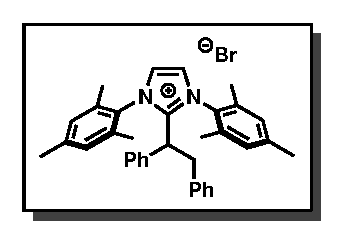
\includegraphics[scale=0.8, angle=90]{chp_alkylation/images/xcaf}
\end{textblock}
\clearpage
%%%
\begin{textblock}{20}(0,0)
\begin{figure}[htb]
\caption{$^{13}$C NMR of  \CMPxcaf\ (\ref{cmp:xcaf})}
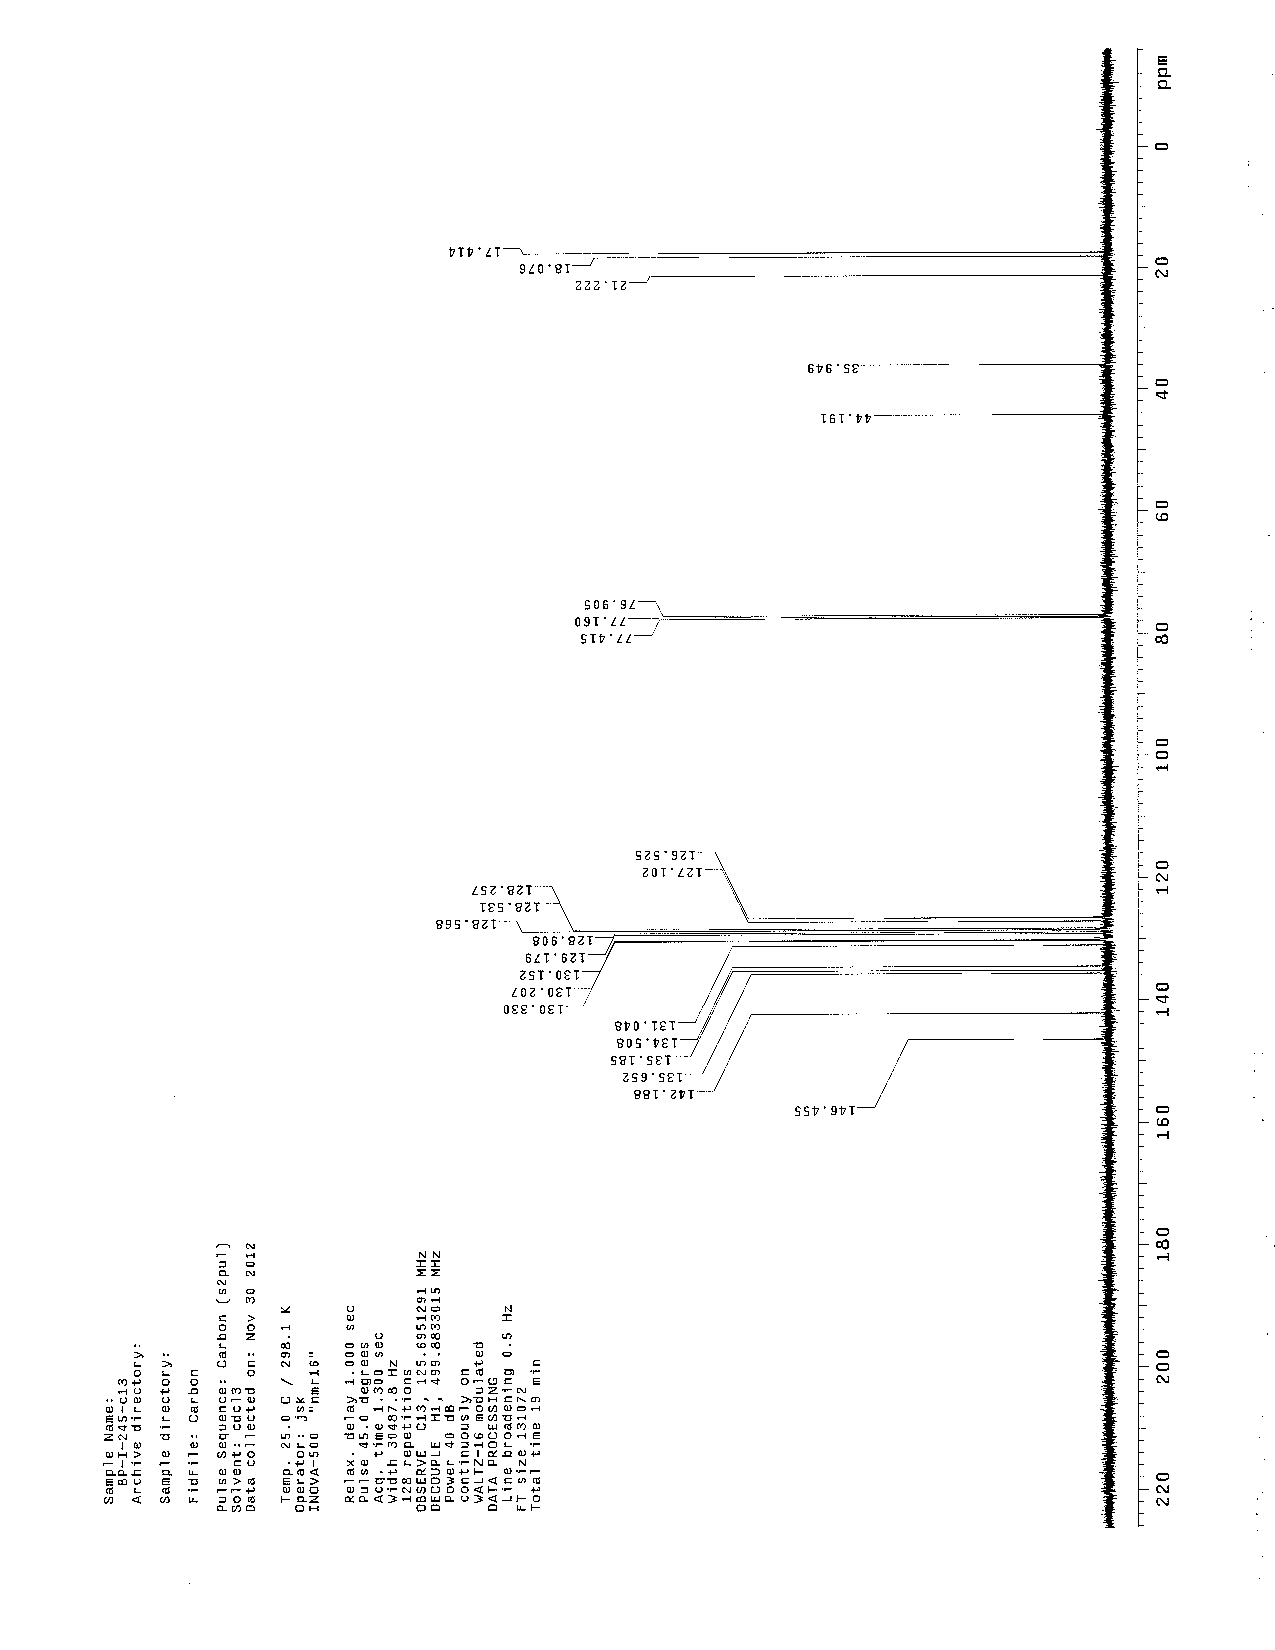
\includegraphics[scale=0.75, trim = 0mm 0mm 0mm 5mm,
clip]{chp_alkylation/images/nmr/xcafC}
\vspace{-100pt}
\end{figure}
\end{textblock}
\begin{textblock}{1}(2,1)
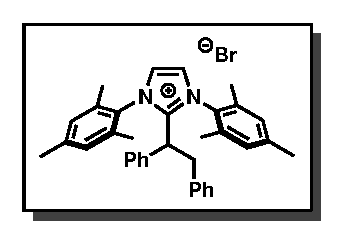
\includegraphics[scale=0.8, angle=90]{chp_alkylation/images/xcaf}
\end{textblock}
\clearpage
%=-=-=-=-=-=-=-=-=-=-=-=-=-=-=-=-=-=-=-=-=-=-=-=-=-=-=-=-=-=-=-=-=-=-=-=-=-=-=-=-=

%=[xcag]=-=-=-=-=-=-=-=-=-=-=-=-=-=-=-=-=-=-=-=-=-=-=-=-=-=-=-=-=-=-=-=-=-=-=-=-=-=-=
\begin{textblock}{20}(0,0)
\begin{figure}[htb]
\caption{$^1$H NMR of \CMPxcag\ (\ref{cmp:xcag})}
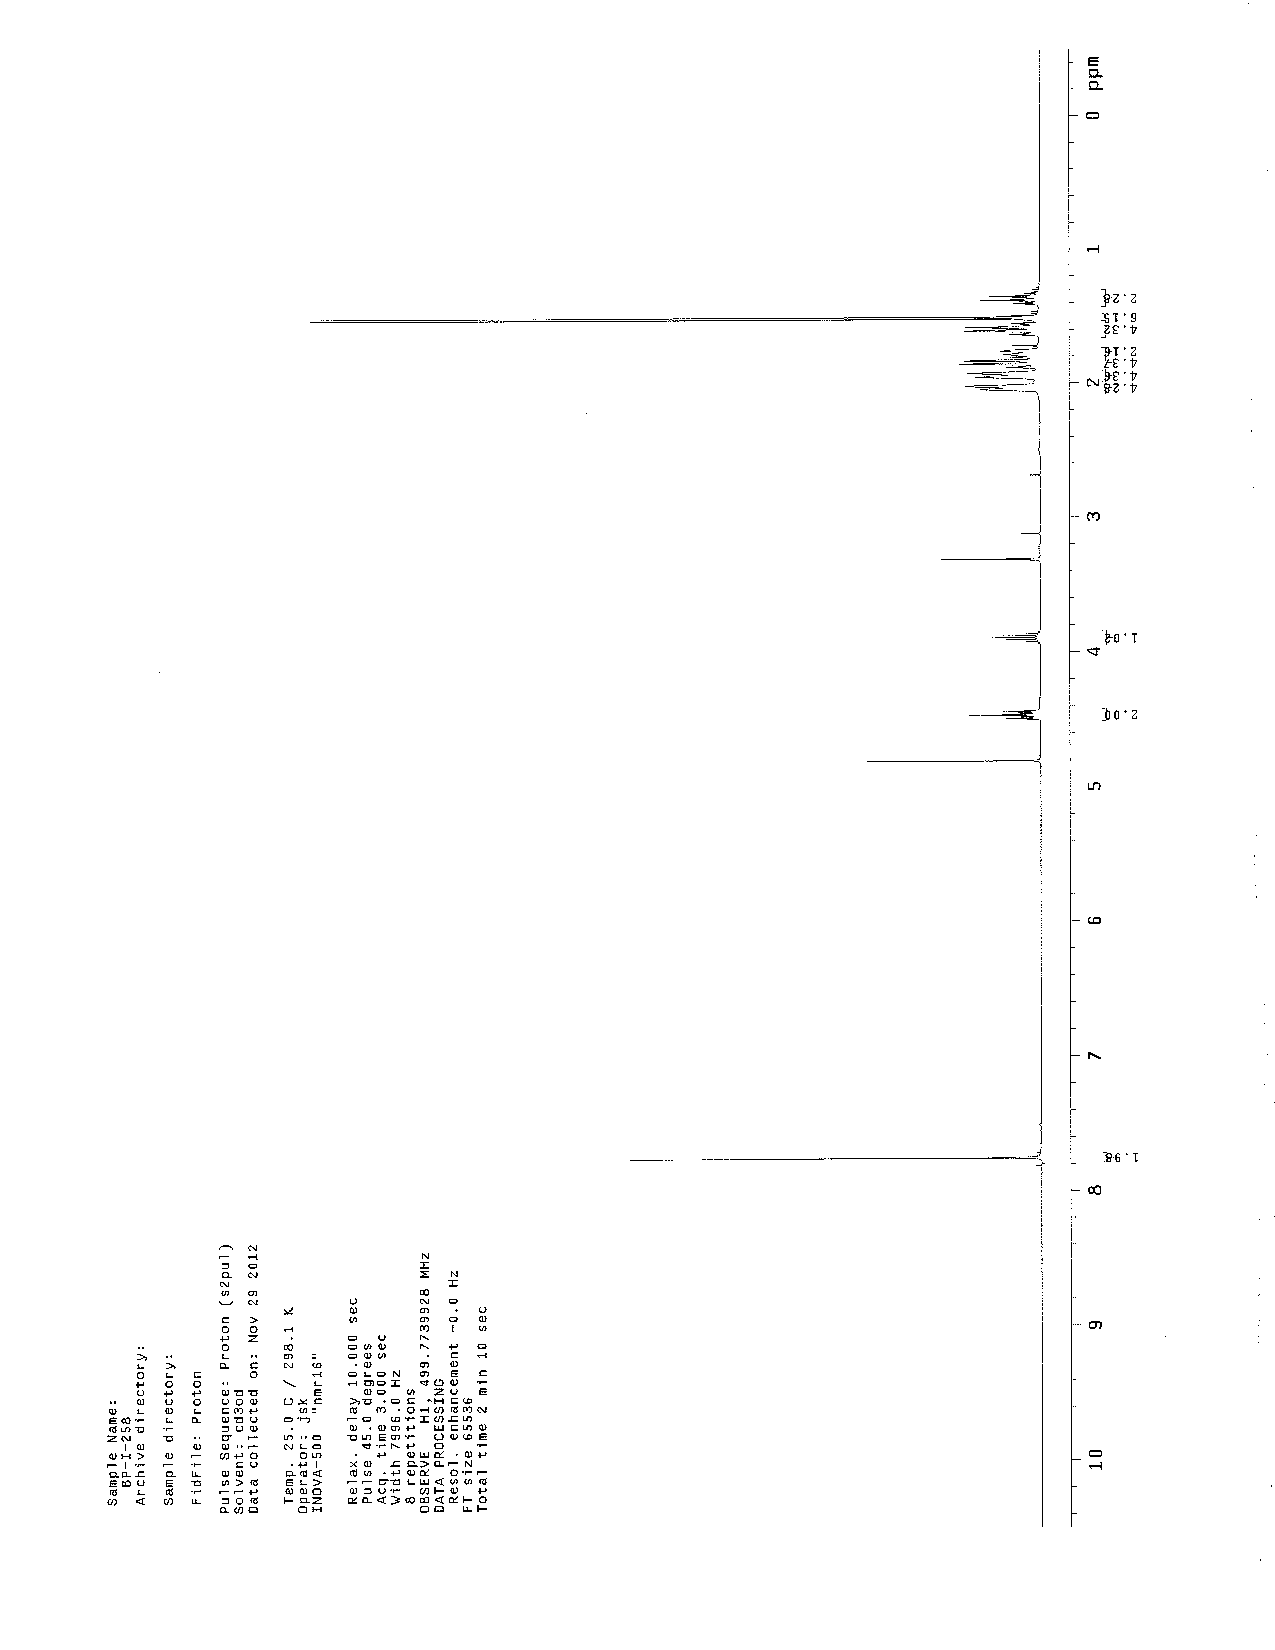
\includegraphics[scale=0.75, trim = 0mm 0mm 0mm 5mm,
clip]{chp_alkylation/images/nmr/xcagH}
\vspace{-100pt}
\end{figure}
\end{textblock}
\begin{textblock}{1}(2,1)
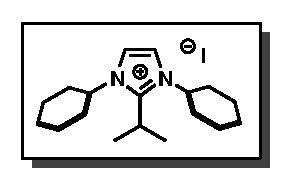
\includegraphics[scale=0.8, angle=90]{chp_alkylation/images/xcag}
\end{textblock}
\clearpage
%%%
\begin{textblock}{20}(0,0)
\begin{figure}[htb]
\caption{$^{13}$C NMR of  \CMPxcag\ (\ref{cmp:xcag})}
\includegraphics[scale=0.75, trim = 0mm 0mm 0mm 5mm,
clip]{chp_alkylation/images/nmr/xcagC}
\vspace{-100pt}
\end{figure}
\end{textblock}
\begin{textblock}{1}(2,10)
\includegraphics[scale=0.8, angle=90]{chp_alkylation/images/xcag}
\end{textblock}
\clearpage
%=-=-=-=-=-=-=-=-=-=-=-=-=-=-=-=-=-=-=-=-=-=-=-=-=-=-=-=-=-=-=-=-=-=-=-=-=-=-=-=-=

%=[xcah]=-=-=-=-=-=-=-=-=-=-=-=-=-=-=-=-=-=-=-=-=-=-=-=-=-=-=-=-=-=-=-=-=-=-=-=-=-=-=
\begin{textblock}{20}(0,0)
\begin{figure}[htb]
\caption{$^1$H NMR of \CMPxcah\ (\ref{cmp:xcah})}
\includegraphics[scale=0.75, trim = 0mm 0mm 0mm 5mm,
clip]{chp_alkylation/images/nmr/xcahH}
\vspace{-100pt}
\end{figure}
\end{textblock}
\begin{textblock}{1}(2,1)
\includegraphics[scale=0.8, angle=90]{chp_alkylation/images/xcah}
\end{textblock}
\clearpage
%%%
\begin{textblock}{20}(0,0)
\begin{figure}[htb]
\caption{$^{13}$C NMR of  \CMPxcah\ (\ref{cmp:xcah})}
\includegraphics[scale=0.75, trim = 0mm 0mm 0mm 5mm,
clip]{chp_alkylation/images/nmr/xcahC}
\vspace{-100pt}
\end{figure}
\end{textblock}
\begin{textblock}{1}(2,10)
\includegraphics[scale=0.8, angle=90]{chp_alkylation/images/xcah}
\end{textblock}
\clearpage
%=-=-=-=-=-=-=-=-=-=-=-=-=-=-=-=-=-=-=-=-=-=-=-=-=-=-=-=-=-=-=-=-=-=-=-=-=-=-=-=-=

%=[xcai]=-=-=-=-=-=-=-=-=-=-=-=-=-=-=-=-=-=-=-=-=-=-=-=-=-=-=-=-=-=-=-=-=-=-=-=-=-=-=
\begin{textblock}{20}(0,0)
\begin{figure}[htb]
\caption{$^1$H NMR of \CMPxcai\ (\ref{cmp:xcai})}
\includegraphics[scale=0.75, trim = 0mm 0mm 0mm 5mm,
clip]{chp_alkylation/images/nmr/xcaiH}
\vspace{-100pt}
\end{figure}
\end{textblock}
\begin{textblock}{1}(2,1)
\includegraphics[scale=0.8, angle=90]{chp_alkylation/images/xcai}
\end{textblock}
\clearpage
%%%
\begin{textblock}{20}(0,0)
\begin{figure}[htb]
\caption{$^{13}$C NMR of  \CMPxcai\ (\ref{cmp:xcai})}
\includegraphics[scale=0.75, trim = 0mm 0mm 0mm 5mm,
clip]{chp_alkylation/images/nmr/xcaiC}
\vspace{-100pt}
\end{figure}
\end{textblock}
\begin{textblock}{1}(2,8.5)
\includegraphics[scale=0.8, angle=90]{chp_alkylation/images/xcai}
\end{textblock}
\clearpage
%=-=-=-=-=-=-=-=-=-=-=-=-=-=-=-=-=-=-=-=-=-=-=-=-=-=-=-=-=-=-=-=-=-=-=-=-=-=-=-=-=

%=[xcaj]=-=-=-=-=-=-=-=-=-=-=-=-=-=-=-=-=-=-=-=-=-=-=-=-=-=-=-=-=-=-=-=-=-=-=-=-=-=-=
\begin{textblock}{20}(0,0)
\begin{figure}[htb]
\caption{$^1$H NMR of \CMPxcaj\ (\ref{cmp:xcaj})}
\includegraphics[scale=0.75, trim = 0mm 0mm 0mm 5mm,
clip]{chp_alkylation/images/nmr/xcajH}
\vspace{-100pt}
\end{figure}
\end{textblock}
\begin{textblock}{1}(2,1)
\includegraphics[scale=0.8, angle=90]{chp_alkylation/images/xcaj}
\end{textblock}
\clearpage
%%%
\begin{textblock}{20}(0,0)
\begin{figure}[htb]
\caption{$^{13}$C NMR of  \CMPxcaj\ (\ref{cmp:xcaj})}
\includegraphics[scale=0.75, trim = 0mm 0mm 0mm 5mm,
clip]{chp_alkylation/images/nmr/xcajC}
\vspace{-100pt}
\end{figure}
\end{textblock}
\begin{textblock}{1}(1,9)
\includegraphics[scale=0.8, angle=90]{chp_alkylation/images/xcaj}
\end{textblock}
\clearpage
%=-=-=-=-=-=-=-=-=-=-=-=-=-=-=-=-=-=-=-=-=-=-=-=-=-=-=-=-=-=-=-=-=-=-=-=-=-=-=-=-=

%=[xcak]=-=-=-=-=-=-=-=-=-=-=-=-=-=-=-=-=-=-=-=-=-=-=-=-=-=-=-=-=-=-=-=-=-=-=-=-=-=-=
\begin{textblock}{20}(0,0)
\begin{figure}[htb]
\caption{$^1$H NMR of \CMPxcak\ (\ref{cmp:xcak})}
\includegraphics[scale=0.75, trim = 0mm 0mm 0mm 5mm,
clip]{chp_alkylation/images/nmr/xcakH}
\vspace{-100pt}
\end{figure}
\end{textblock}
\begin{textblock}{1}(2,1)
\includegraphics[scale=0.8, angle=90]{chp_alkylation/images/xcak}
\end{textblock}
\clearpage
%%%
\begin{textblock}{20}(0,0)
\begin{figure}[htb]
\caption{$^{13}$C NMR of  \CMPxcak\ (\ref{cmp:xcak})}
\includegraphics[scale=0.75, trim = 0mm 0mm 0mm 5mm,
clip]{chp_alkylation/images/nmr/xcakC}
\vspace{-100pt}
\end{figure}
\end{textblock}
\begin{textblock}{1}(2,1)
\includegraphics[scale=0.8, angle=90]{chp_alkylation/images/xcak}
\end{textblock}
\clearpage
%=-=-=-=-=-=-=-=-=-=-=-=-=-=-=-=-=-=-=-=-=-=-=-=-=-=-=-=-=-=-=-=-=-=-=-=-=-=-=-=-=

%=[xcal]=-=-=-=-=-=-=-=-=-=-=-=-=-=-=-=-=-=-=-=-=-=-=-=-=-=-=-=-=-=-=-=-=-=-=-=-=-=-=
\begin{textblock}{20}(0,0)
\begin{figure}[htb]
\caption{$^1$H NMR of \CMPxcal\ (\ref{cmp:xcal})}
\includegraphics[scale=0.75, trim = 0mm 0mm 0mm 5mm,
clip]{chp_alkylation/images/nmr/xcalH}
\vspace{-100pt}
\end{figure}
\end{textblock}
\begin{textblock}{1}(2,1)
\includegraphics[scale=0.8, angle=90]{chp_alkylation/images/xcal}
\end{textblock}
\clearpage
%%%
\begin{textblock}{20}(0,0)
\begin{figure}[htb]
\caption{$^{13}$C NMR of  \CMPxcal\ (\ref{cmp:xcal})}
\includegraphics[scale=0.75, trim = 0mm 0mm 0mm 5mm,
clip]{chp_alkylation/images/nmr/xcalC}
\vspace{-100pt}
\end{figure}
\end{textblock}
\begin{textblock}{1}(2,1)
\includegraphics[scale=0.8, angle=90]{chp_alkylation/images/xcal}
\end{textblock}
\clearpage
%%%
\begin{textblock}{20}(0,0)
\begin{figure}[htb]
\caption{HSQC NMR of  \CMPxcal\ (\ref{cmp:xcal})}
\includegraphics[scale=0.75, trim = 0mm 0mm 0mm 5mm,
clip]{chp_alkylation/images/nmr/xcalHSQC}
\vspace{-100pt}
\end{figure}
\end{textblock}
\begin{textblock}{1}(1,1)
\includegraphics[scale=0.8, angle=90]{chp_alkylation/images/xcal}
\end{textblock}
\clearpage
%=-=-=-=-=-=-=-=-=-=-=-=-=-=-=-=-=-=-=-=-=-=-=-=-=-=-=-=-=-=-=-=-=-=-=-=-=-=-=-=-=

%=[xcam]=-=-=-=-=-=-=-=-=-=-=-=-=-=-=-=-=-=-=-=-=-=-=-=-=-=-=-=-=-=-=-=-=-=-=-=-=-=-=
\begin{textblock}{20}(0,0)
\begin{figure}[htb]
\caption{$^1$H NMR of \CMPxcam\ (\ref{cmp:xcam})}
\includegraphics[scale=0.75, trim = 0mm 0mm 0mm 5mm,
clip]{chp_alkylation/images/nmr/xcamH}
\vspace{-100pt}
\end{figure}
\end{textblock}
\begin{textblock}{1}(2,1)
\includegraphics[scale=0.8, angle=90]{chp_alkylation/images/xcam}
\end{textblock}
\clearpage
%%%
\begin{textblock}{20}(0,0)
\begin{figure}[htb]
\caption{$^{13}$C NMR of  \CMPxcam\ (\ref{cmp:xcam})}
\includegraphics[scale=0.75, trim = 0mm 0mm 0mm 5mm,
clip]{chp_alkylation/images/nmr/xcamC}
\vspace{-100pt}
\end{figure}
\end{textblock}
\begin{textblock}{1}(0,1)
\includegraphics[scale=0.8, angle=90]{chp_alkylation/images/xcam}
\end{textblock}
\clearpage
%=-=-=-=-=-=-=-=-=-=-=-=-=-=-=-=-=-=-=-=-=-=-=-=-=-=-=-=-=-=-=-=-=-=-=-=-=-=-=-=-=

%=[xcan]=-=-=-=-=-=-=-=-=-=-=-=-=-=-=-=-=-=-=-=-=-=-=-=-=-=-=-=-=-=-=-=-=-=-=-=-=-=-=
\begin{textblock}{20}(0,0)
\begin{figure}[htb]
\caption{$^1$H NMR of \CMPxcan\ (\ref{cmp:xcan})}
\includegraphics[scale=0.75, trim = 0mm 0mm 0mm 5mm,
clip]{chp_alkylation/images/nmr/xcanH}
\vspace{-100pt}
\end{figure}
\end{textblock}
\begin{textblock}{1}(2,1)
\includegraphics[scale=0.8, angle=90]{chp_alkylation/images/xcan}
\end{textblock}
\clearpage
%%%
\begin{textblock}{20}(0,0)
\begin{figure}[htb]
\caption{$^{13}$C NMR of  \CMPxcan\ (\ref{cmp:xcan})}
\includegraphics[scale=0.75, trim = 0mm 0mm 0mm 5mm,
clip]{chp_alkylation/images/nmr/xcanC}
\vspace{-100pt}
\end{figure}
\end{textblock}
\begin{textblock}{1}(2,1)
\includegraphics[scale=0.8, angle=90]{chp_alkylation/images/xcan}
\end{textblock}
\clearpage
%=-=-=-=-=-=-=-=-=-=-=-=-=-=-=-=-=-=-=-=-=-=-=-=-=-=-=-=-=-=-=-=-=-=-=-=-=-=-=-=-=

%=[xcana]=-=-=-=-=-=-=-=-=-=-=-=-=-=-=-=-=-=-=-=-=-=-=-=-=-=-=-=-=-=-=-=-=-=-=-=-=-=-=
\begin{textblock}{20}(0,0)
\begin{figure}[htb]
\caption{$^1$H NMR of \CMPxcana\ (\ref{cmp:xcana})}
\includegraphics[scale=0.75, trim = 0mm 0mm 0mm 5mm,
clip]{chp_alkylation/images/nmr/xcanaH}
\vspace{-100pt}
\end{figure}
\end{textblock}
\begin{textblock}{1}(2,1)
\includegraphics[scale=0.8, angle=90]{chp_alkylation/images/xcana}
\end{textblock}
\clearpage
%%%
\begin{textblock}{20}(0,0)
\begin{figure}[htb]
\caption{$^{13}$C NMR of  \CMPxcana\ (\ref{cmp:xcana})}
\includegraphics[scale=0.75, trim = 0mm 0mm 0mm 5mm,
clip]{chp_alkylation/images/nmr/xcanaC}
\vspace{-100pt}
\end{figure}
\end{textblock}
\begin{textblock}{1}(2,1)
\includegraphics[scale=0.8, angle=90]{chp_alkylation/images/xcana}
\end{textblock}
\clearpage
%=-=-=-=-=-=-=-=-=-=-=-=-=-=-=-=-=-=-=-=-=-=-=-=-=-=-=-=-=-=-=-=-=-=-=-=-=-=-=-=-=

%=[xcanb]=-=-=-=-=-=-=-=-=-=-=-=-=-=-=-=-=-=-=-=-=-=-=-=-=-=-=-=-=-=-=-=-=-=-=-=-=-=-=
\begin{textblock}{20}(0,0)
\begin{figure}[htb]
\caption{$^1$H NMR of \CMPxcanb\ (\ref{cmp:xcanb})}
\includegraphics[scale=0.75, trim = 0mm 0mm 0mm 5mm,
clip]{chp_alkylation/images/nmr/xcanbH}
\vspace{-100pt}
\end{figure}
\end{textblock}
\begin{textblock}{1}(2,1)
\includegraphics[scale=0.8, angle=90]{chp_alkylation/images/xcanb}
\end{textblock}
\clearpage
%%%
\begin{textblock}{20}(0,0)
\begin{figure}[htb]
\caption{$^{13}$C NMR of  \CMPxcanb\ (\ref{cmp:xcanb})}
\includegraphics[scale=0.75, trim = 0mm 0mm 0mm 5mm,
clip]{chp_alkylation/images/nmr/xcanbC}
\vspace{-100pt}
\end{figure}
\end{textblock}
\begin{textblock}{1}(2,1)
\includegraphics[scale=0.8, angle=90]{chp_alkylation/images/xcanb}
\end{textblock}
\clearpage
%=-=-=-=-=-=-=-=-=-=-=-=-=-=-=-=-=-=-=-=-=-=-=-=-=-=-=-=-=-=-=-=-=-=-=-=-=-=-=-=-=
			% NMR spectroscopy data